% !TeX program = pdflatex
% Revision working source. Numerical evidence is generated only from saved runs.
\documentclass[software,article,submit,moreauthors]{Definitions/mdpi}
\firstpage{1}
\pubvolume{1}
\issuenum{1}
\articlenumber{0}
\pubyear{2026}
\copyrightyear{2026}
\hreflink{}
\doinum{}
\datereceived{}
\daterevised{}
\dateaccepted{}
\datepublished{}
\renewcommand{\papercitation}{Manuscript submitted to Software.}
\usepackage{amsmath,amssymb,amsthm,graphicx,booktabs,algorithm,algorithmic,url}
\graphicspath{{figures/}}
\setlength{\emergencystretch}{2em}
\newcommand{\CE}{\mathcal{L}_{\mathrm{CE}}}
\newcommand{\Drs}{D_{rs}}

\Title{Fed-EMNU: Federated Error-Maximizing Noise for Approximate Class Suppression}
\Author{Jiale Wang $^{1}$, Zixiao Liu $^{2}$ and Jianhua Wang $^{3,}$*}
\AuthorNames{Jiale Wang, Zixiao Liu and Jianhua Wang}
\address{$^{1}$ \quad College of Intelligent Systems Science and Engineering,
Harbin Engineering University, Harbin 150001, China; wangjiale03082006@163.com\\
$^{2}$ \quad College of Software, Taiyuan University of Technology, Taiyuan
030021, China; 2024006625@link.tyut.edu.cn\\
$^{3}$ \quad School of Computer Science and Technology (Big Data Institute),
Taiyuan University of Technology, Taiyuan 030021, China;
wangjianhua02@tyut.edu.cn\\
$*$ \quad Correspondence: wangjianhua02@tyut.edu.cn}

\abstract{The ``Right to be Forgotten'' has spurred interest in machine
unlearning (MU), enabling data owners to request removal of their data's
influence from trained models. While many MU methods focus on centralized
settings, federated learning (FL) introduces distributed ownership and limited
data access. Our contribution is an implementation-oriented federated adaptation and empirical
characterization, rather than a new optimization principle or a claim of superiority
over UNSIR or PAR. We study Fed-EMNU, a class-level federated adaptation of prior
error-maximizing-noise impair--repair methods. The server generates synthetic
inputs; affected clients perform local unlearning and enhancement using
retained data before server aggregation. Five-seed CIFAR-10 experiments yield
forget accuracy of $6.80\pm1.35$\% and retained accuracy of $75.24\pm0.08$\%
under IID partitions, with a paired retraining-to-method compute-time ratio of
$21.54\pm0.35$. The UNSIR-style adaptation is faster and has lower target-class
accuracy, while Fed-EMNU has higher mean retained accuracy. The main comparison
uses all retained data; separate matched half-subset experiments do not support
a confidence-ranking advantage over random selection. Non-IID and additional
dataset, architecture, client-count and request/training-horizon studies expose
limits of the fixed recipe. A PAR-code-based comparison is reported with its
adaptation boundary. New three-seed controls at matched update budgets do
not support a consistent retained-utility advantage of the Fed-EMNU noise
penalty. Optimized noise lowers the declared target attack AUC relative to
Gaussian inputs but has mixed accuracy effects; event weighting shows a limited utility--suppression
trade-off. Additional comparisons under common maximum wall-clock caps of 10--40 seconds,
with actual execution time measured separately, show
higher mean retained utility alongside higher target accuracy and attack AUC,
without uniform superiority. Residual target behavior and membership differences from
retraining restrict the method to approximate class suppression, without a
formal privacy or deletion guarantee. The original implementation is available
at \url{https://github.com/Daoge12/Fed-EMNU}.}
\keyword{federated learning; approximate unlearning; class revocation;
error-maximizing noise; retained-data selection}

\begin{document}

\fancypagestyle{plain}{\fancyhf{}
\fancyfoot[L]{\footnotesize Version \today\ submitted to \emph{Software}}
\fancyfoot[R]{\footnotesize Revised manuscript}
\renewcommand{\footrulewidth}{0.4pt}}
\rfoot{\footnotesize Revised manuscript}
\maketitle
\section{Introduction}


With the widespread adoption of machine learning technologies in fields such as
economics, healthcare, energy, and industry, an increasing amount of data has
been utilized to train intelligent models. However, these data often contain a
substantial amount of personal and sensitive information. In recent years, the
proposal of the Right to be Forgotten \cite{ref1} has drawn renewed attention to
data controllability and privacy protection, giving rise to the emerging
research paradigm of machine unlearning. Machine unlearning aims to empower
users with the ability to request removal of their personal data's influence
from public datasets or pre-trained models, while maintaining the model's
performance on the remaining tasks as much as possible.

In this paper, we conduct research on model training and unlearning under the
premise that raw data are not shared. Specifically, we focus on the Federated
Learning (FL) \cite{ref2,ref3,ref4,ref5,ref6,ref7} framework---a distributed
machine learning paradigm that allows multiple clients to keep their private
data locally while participating in global model training by uploading only
model parameters or gradients. This mechanism enables cross-domain collaborative modeling without sharing raw
examples, but does not itself guarantee privacy against inference or gradient
reconstruction attacks. However, the non-sharing nature of
data also introduces new challenges for model updating and unlearning, making it
more difficult to efficiently remove the influence of designated data while
preserving privacy.

Removing specific data samples from a pre-trained federated learning (FL) model
can be naively approached by retraining a new model from scratch on the
remaining dataset, excluding the target samples. However, for real-world models
trained over long periods with large datasets, this strategy can be
computationally expensive.

There are two main strategies for achieving unlearning without naively
retraining the model---exact unlearning and approximate unlearning. Exact unlearning aims to match the distribution of models obtained by
retraining without the requested records, under the assumptions of the learning
procedure. This is stronger than low target-class prediction accuracy. Previous studies
\cite{ref8,ref9,ref10,ref11,ref12} have proposed machine unlearning methods for
structured model classes, including linear and tree-based models. Their
assumptions do not automatically extend to deep federated networks\cite{ref13}.

The goal of approximate unlearning is to improve the efficiency of machine
unlearning \cite{ref8,ref14}, by minimizing the impact of specific data samples,
though it may not fully eliminate their influence. This process is typically
achieved through approximate methods, which may sacrifice precision in exchange
for reduced computational cost. Related approaches\cite{ref13,ref15,ref16} have different model, data-access
and update-history requirements; these must be stated when comparing methods. However, studies have shown that attackers
can exploit gradients uploaded by clients, such as through gradient leakage
attacks \cite{ref17,ref18}. Consequently, data locality and computational efficiency must be distinguished
from privacy guarantees.

In the case of Independent and Identically Distributed (IID) data, local
retained subsets may more closely represent the global distribution. Due to the consistent
data distribution, the model after the unlearning operation can maintain
relatively stable performance across most classes. However, despite this, the
model may still experience slight accuracy degradation during the unlearning
process, especially when large-scale adjustments are required. The magnitude of any accuracy change and the remaining membership information
must be measured, rather than inferred from the partition type.

In contrast, the challenges of approximate unlearning are more pronounced in the
case of Non-IID (Non-Independent and Identically Distributed) data. In this
scenario, the distribution of data samples varies significantly across different
clients, meaning that the model may rely more heavily on features from specific
subsets of data for certain classes. During approximate unlearning, it may not
be possible to completely remove the influence of certain class data, resulting
in a noticeable decline in model performance for some classes after unlearning.
This is particularly true when the data for the class to be forgotten has a
significant impact on the model during training, and the Non-IID nature of the
data makes it difficult to effectively eliminate this influence, leading to
reduced generalization ability on other classes.


To study alternatives to retained-data retraining, we evaluate Fed-EMNU as a
specified federated adaptation of existing error-maximizing-noise and
impair--repair techniques. UNSIR~\cite{ref20} supplies the underlying noise-based
mechanism, and PAR~\cite{ref21} already combines perturbation and restoration
in a federated setting. Our scientific question is whether the particular
noise objective, local update budget and affected-client aggregation used here
produce a useful suppression--utility--cost trade-off. Combining these elements
does not by itself establish a new optimization principle or a deletion guarantee.

\textbf{The contributions and their evidence boundaries are as follows:}
\begin{itemize}
\item We specify an implementable federated class-suppression protocol,
including request scope, synthetic labels, a shared request-time checkpoint,
client-local updates and retained-count-weighted aggregation. This is a
workflow specification and adaptation of prior mechanisms; requester-level
scope is defined but only global class requests are experimentally evaluated.
\item We examine the recipe's components with stage-removal controls,
noise-optimization and event-weighting controls, and within-budget comparisons
of the two noise objectives. These experiments test particular implementation
choices rather than assuming integration is beneficial. Confidence-ranked
selection is an optional mechanism whose advantage is not supported by the
matched subset results.
\item We provide reference-based measurements of target suppression, retained
utility, membership behavior and compute time, together with explicit failure
cases across datasets, heterogeneity and client counts. The released
configurations, numerical metrics, frozen source snapshots and replay scripts
support inspection and regeneration
of the empirical findings; reproducibility is not evidence of algorithmic novelty.
\end{itemize}

Section 2 describes Fed-EMNU and its relationship to the closest methods.
Section 3 evaluates the framework and reports the additional studies. Section 4
presents the conclusions and limitations.

\section{Methodology}
\label{sec:method}

Upon receiving an unlearning request for a specific class, the server generates
optimized noise against the request-time model. The noise is combined with a
selected portion of remaining local data for unlearning, followed by enhancement
on the same retained subset. Below we clarify the objective, labels, selection
and server update needed to make this process reproducible.

\subsection{Problem Statement}
\label{sec:scope}
Let $D=\bigcup_{i=1}^{M}D_i$ denote disjoint client training datasets with labels
in $\mathcal{Y}=\{0,\ldots,K-1\}$. A trained global model has parameters
$\theta_0$ and posterior vector $p_{\theta_0}(\cdot\mid x)$. A request specifies
target classes $\mathcal{Y}_f$ and a set of affected clients $A$. Define
\begin{equation}
D_{f,i}=\begin{cases}\{(x,y)\in D_i:y\in\mathcal{Y}_f\},&i\in A,\\
\emptyset,&i\notin A,\end{cases}
\qquad D_{r,i}=D_i\setminus D_{f,i}.
\label{eq:request}
\end{equation}
For global class revocation, $A$ includes every client holding the target class;
the requested records are removed across the federation. For requester-level
revocation, $A=\{q\}$ contains only the requesting client. The latter does not
remove other clients' records in the same class, so low global target-class
accuracy is not its defining success criterion.

Write $\theta^{-f}=\operatorname{Train}(\{D_{r,i}\},\xi)$ for a reference
obtained from a fresh random initialization using a recorded training procedure
and seed $\xi$. It uses the original partition and client schedule, omits exactly
the requested records, and has a disclosed fixed training budget. It never starts
from $\theta_0$. Independent training randomness makes it a stochastic reference;
one reference draw cannot establish equality of model distributions.

The approximate output $\theta'$ is assessed by retained utility and behavioral
similarity to $\theta^{-f}$. We do not impose a uniform target-class probability
on every input while simultaneously fixing all retained-class probabilities:
those constraints may conflict with posterior normalization and are unnecessary
for the reference-based evaluation.

\subsection{Federated Error-Maximizing Noise Unlearning}
\label{sec:protocol}
As shown in Figure~\ref{fig:overview}, Fed-EMNU generates error-maximizing noise
and combines it with remaining data for local training. The server distributes
the same request checkpoint to all affected clients, then aggregates their
returned states. All participating clients therefore update a common starting
model within the same coordinated event.

During pretraining, a recorded subset $S_t$ participates in round $t$. Clients
start from the same round checkpoint, perform the configured local optimization,
and send their states to the server. Floating-point states are aggregated as
\begin{equation}
\theta_{t+1}=\sum_{i\in S_t}\frac{|D_i|}{\sum_{j\in S_t}|D_j|}
\theta_{t+1}^{(i)}.
\label{eq:fedavg}
\end{equation}
Each local call initializes a fresh Adam optimizer; optimizer moments are not
transmitted or carried between rounds. Local data are shuffled using recorded
seeds. The standard ResNet stem reduces a $32\times32$ input to a $1\times1$
final feature map. If a last minibatch has one example, the implementation uses
stored batch-normalization statistics for that minibatch while still updating
parameters, rather than discarding the example or estimating an undefined
single-example variance.
Batch-normalization integer counters use the maximum participating counter and
are recorded as state rather than averaged parameters. The sample-weighted
protocol is an explicit revision from the supplied implementation's equal
client weighting. Results from the two protocols must not be combined.

For an unlearning event, the server freezes a request-time checkpoint
$\theta_0$. It generates one synthetic batch per target class and sends the
checkpoint and batches to every affected client with target examples. Each
client independently performs selection, impair, and repair from this same
checkpoint. The server replaces its current state with
\begin{equation}
\theta'=\sum_{i\in A_f}\frac{|D_{r,i}|}{\sum_{j\in A_f}|D_{r,j}|}
\theta_i', \qquad A_f=\{i\in A:|D_{f,i}|>0\}.
\label{eq:unlearnagg}
\end{equation}
This is a heuristic state update, not an algebraic subtraction of historical
contributions. When $|A_f|=1$, the returned state directly replaces the global
state. All affected clients must be available in the evaluated global-class
protocol. Handling unavailable clients or asynchronous requests is outside the
evaluated setting.

When some clients hold no target examples, Equation~\ref{eq:unlearnagg}
normalizes weights over $A_f$ only. The shared starting checkpoint already
contains information learned from all clients; nonparticipation therefore does
not imply that an unaffected client's knowledge is erased. Nevertheless, the
event provides no separate contribution or repair update from those clients,
and the resulting model can be biased toward the retained distributions of
target holders. This limitation is exposed by the sparse-owner setting in
Appendix~\ref{sec:followup}. We evaluate the stated heuristic without claiming
that it preserves unaffected-client utility or implements an exact global
deletion operation.

Later FL rounds can relearn a revoked contribution if those records are reused.
The protocol therefore quarantines requested examples before subsequent
training. Removing a record from the training pool does not prevent learning
related features from other records. Checkpoints and request identifiers must be
tracked to prevent stale unlearning updates from overwriting newer global states.

\begin{figure}[htbp]
\centering
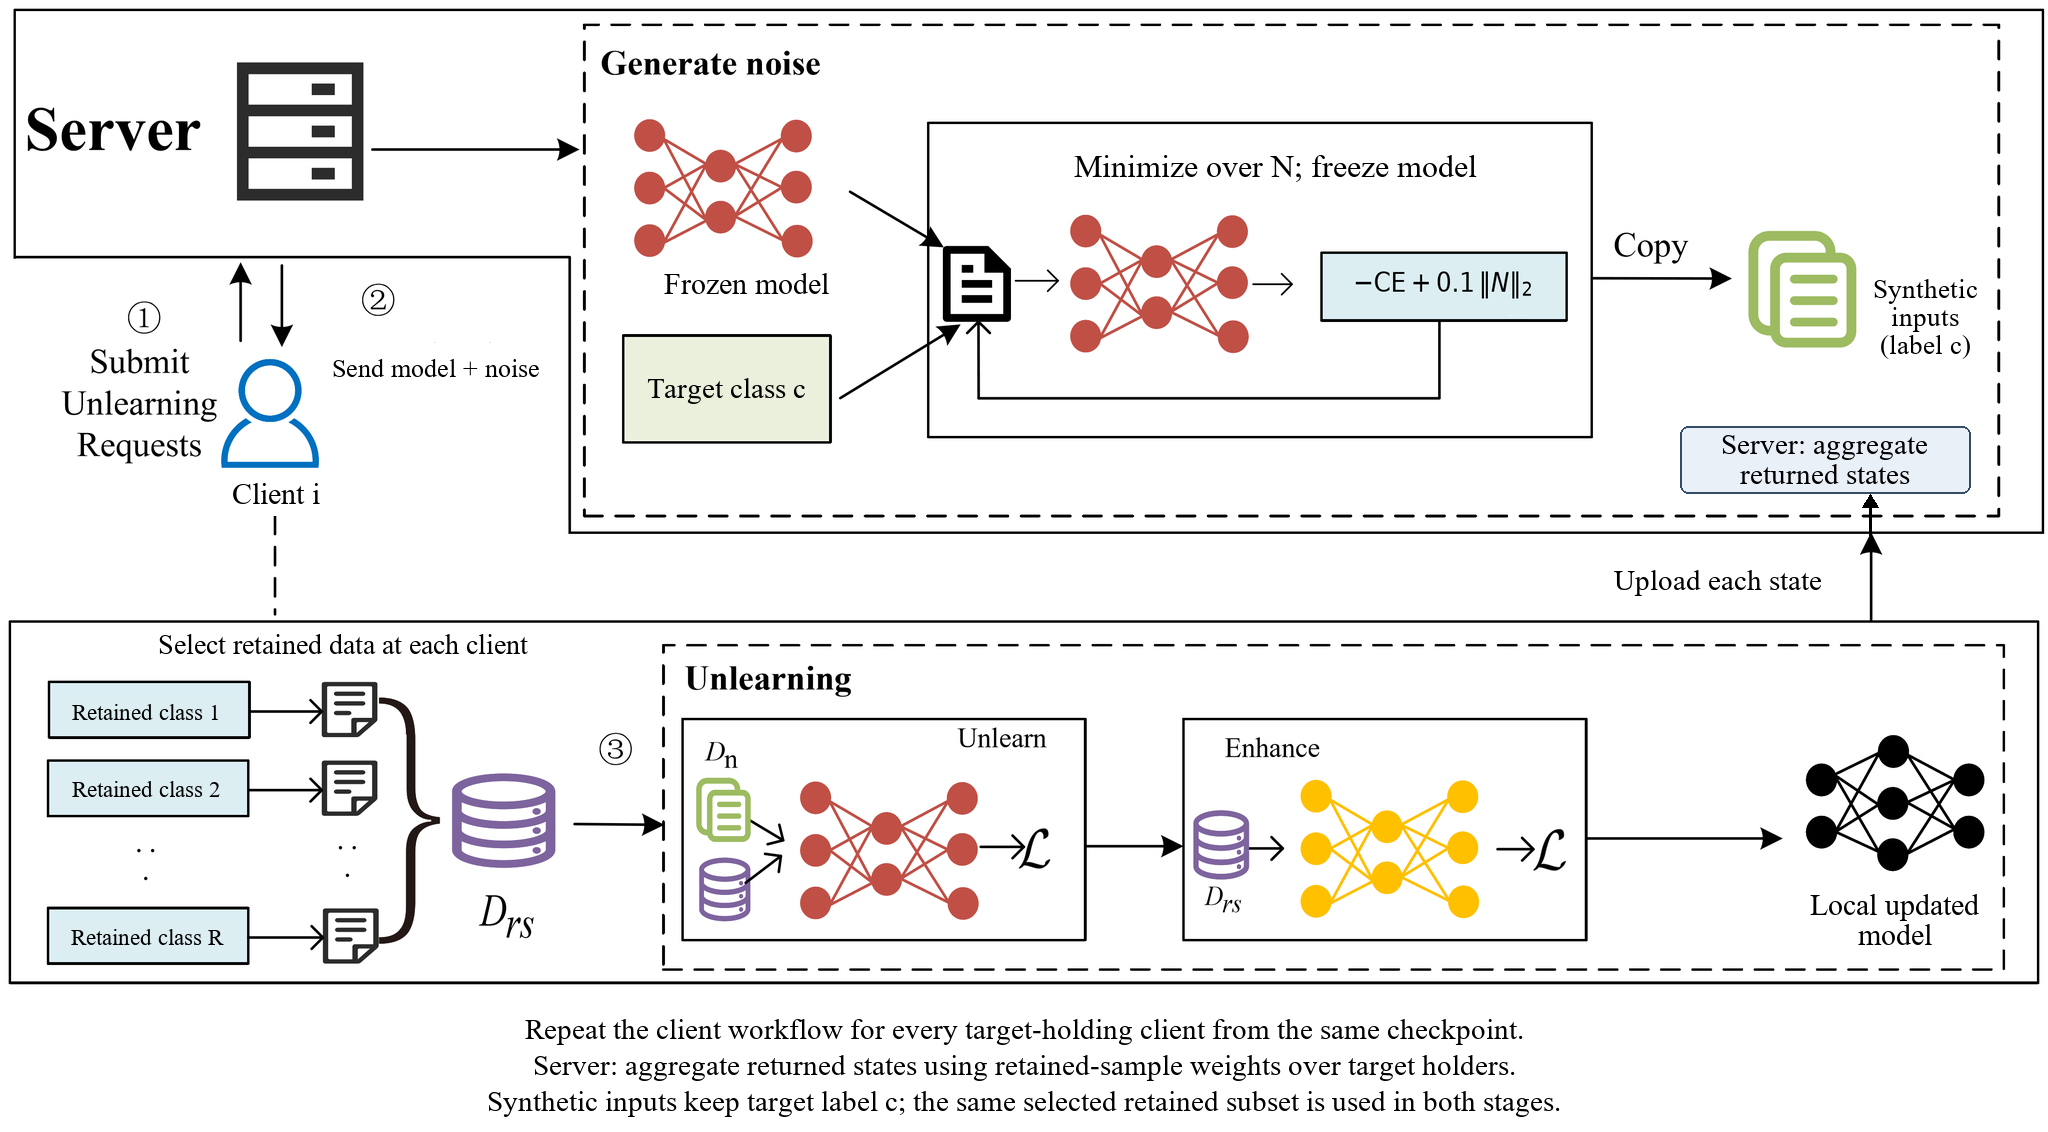
\includegraphics[width=\linewidth]{fig1_overview_revised.png}
\caption{Explicit coordinated global-class event. Every affected client updates
the same request-time checkpoint. Raw local examples remain at clients.
The client workflow is repeated for every target holder; aggregation uses only
those clients as in Equation~\ref{eq:unlearnagg}.}
\label{fig:protocol}\label{fig:overview}
\end{figure}

\subsection{Detail of Fed-EMNU}
\subsubsection{Noise Generation}
\label{sec:noise}
For target class $c$, the server initializes a batch
$N_c\in\mathbb{R}^{B\times3\times32\times32}$ with independent
$\mathcal{N}(0,1)$ entries, with $B=128$, and minimizes over $N$
\begin{equation}
\min_N\; J_c(N)=-\frac1B\sum_{b=1}^{B}\CE(f_{\theta_0}(N_b),c)
+\lambda\|N\|_2.
\label{eq:noise}
\end{equation}
The cross-entropy term is averaged across the batch, and $\|N\|_2$ is the
unsquared Euclidean norm of the flattened full tensor. Adam updates only $N$;
all model parameters and batch-normalization statistics are frozen. The default
noise schedule contains 10 outer iterations of eight Adam steps, learning rate
0.1, and $\lambda=0.1$. There is no hard norm bound, projection, or image-range
clipping. These details match the Fed-EMNU objective under evaluation.

Each synthetic input retains target label $c$ in the impair dataset. The
negative cross-entropy term encourages larger target-class loss under the frozen
model, balanced by the norm penalty; the combined optimization need not increase
cross-entropy monotonically. The subsequent model update minimizes loss on
these synthetic inputs. This drives a parameter
change associated with the target decision region. Retained examples and repair
constrain collateral damage. The mechanism is an empirical heuristic: fitting
synthetic examples with label $c$ does not mathematically imply deletion of the
training influence of real examples with label $c$.

\subsubsection{Local Remaining Dataset Selection}
\label{sec:selection}
The server is responsible for noise generation, while subsequent unlearning is
performed by affected clients. To control local computation, a subset of the
remaining data is selected and reused for unlearning and enhancement.

Each affected client selects a fixed subset $D_{rs,i}\subseteq D_{r,i}$ once per
request and reuses exactly that subset in both impair and repair. For every
nonempty local retained class set $D_{r,i,c}$, the count is
$n_{i,c}=\max(1,\lfloor rt\,|D_{r,i,c}|\rfloor)$, where $0<rt\leq1$.
Random selection draws without replacement separately within each class.

For confidence selection, the client evaluates the received global model
$\theta_0$ in evaluation mode at request time. It traverses its local examples
in deterministic index order and associates each local index $j$ with
$s_{i,j}=\max_k p_{\theta_0}(k\mid x_{i,j})$. For each retained class, the
largest $n_{i,c}$ scores are selected, with local index breaking ties. The score
is the maximum posterior, not necessarily the true-label posterior. Recomputing
it at request time avoids stale local-model scores and missing scores for a
client that skipped recent FL rounds.

High confidence can favor easy examples and misclassified examples with a
confident wrong label. It can under-represent boundary samples and minority
modes. Selection is therefore a utility heuristic, with stratified random
selection as its direct control. The implementation saves exact selected indices
and sample counts, uses no undocumented duplication, and keeps incomplete final
minibatches.

\subsubsection{Unlearning and Enhancement}
\label{sec:updates}
Replicating each optimized batch $r_n$ times produces a synthetic dataset
$D_{n,c}$ of $B r_n$ examples labeled $c$. The default $r_n$ is 20. Each client
performs one impair epoch for each requested target class on
$D_{n,c}\cup D_{rs,i}$, minimizing
\begin{equation}
L_{u,i}(\theta)=\frac{1}{|D_{n,c}|+|D_{rs,i}|}
\sum_{(x,y)\in D_{n,c}\cup D_{rs,i}}\CE(f_\theta(x),y).
\label{eq:impair}
\end{equation}
Minibatches are shuffled and Adam uses learning rate 0.02. Repair then minimizes
\begin{equation}
L_{r,i}(\theta)=\frac{1}{|D_{rs,i}|}
\sum_{(x,y)\in D_{rs,i}}\CE(f_\theta(x),y)
\label{eq:repair}
\end{equation}
for three epochs with Adam at learning rate 0.01. Each impair pass and the repair
stage initialize fresh optimizers. Multi-class requests use a
recorded target order; sequential impair passes are distinct from a joint
multi-class impair pass and are not treated as equivalent. The complete event is
given in Algorithm~\ref{alg:complete}.

\begin{algorithm}[t]
\caption{Fed-EMNU event with explicit request scope}
\label{alg:complete}
\begin{algorithmic}[1]
\REQUIRE Checkpoint $\theta_0$, local sets $D_i$, affected clients $A$, target
classes $\mathcal{Y}_f$, ratio $rt$, seeds and optimization budgets
\ENSURE Updated server state $\theta'$ and audit records
\STATE Define $D_{f,i},D_{r,i}$ using Equation~\ref{eq:request}; quarantine $D_{f,i}$
\FOR{each target class $c$ in the recorded order}
\STATE Initialize $N_c\sim\mathcal{N}(0,1)$; freeze $\theta_0$
\STATE Optimize only $N_c$ using Equation~\ref{eq:noise}; detach optimized inputs
\ENDFOR
\FOR{each affected client $i$ with $|D_{f,i}|>0$}
\STATE Initialize $\theta_i\leftarrow\theta_0$; set $D_{rs,i}\leftarrow\emptyset$
\FOR{each nonempty retained class $c$}
\STATE Construct $D_{r,i,c}$; compute $n_{i,c}$ from its size
\STATE Select $n_{i,c}$ local indices randomly or by request-time confidence
\STATE Add the selected examples to $D_{rs,i}$ and save their indices
\ENDFOR
\FOR{each target class $c$ in the recorded order}
\STATE Label and repeat $N_c$; impair $\theta_i$ for one epoch on $D_{n,c}\cup D_{rs,i}$
\ENDFOR
\STATE Repair $\theta_i$ on the same $D_{rs,i}$ for the configured epochs
\STATE Upload $\theta_i'$ and its retained sample count
\ENDFOR
\STATE Aggregate using Equation~\ref{eq:unlearnagg}; save checkpoint and provenance
\RETURN $\theta'$
\end{algorithmic}
\end{algorithm}

\subsection{Comparison with Closely Related Methods}
\label{sec:related}
\subsubsection{Error-Maximizing Noise and Impair--Repair Updates}


Tarun et al.~\cite{ref20} study centralized class unlearning without access to
the forgotten examples during the update. Their method initializes synthetic
inputs from a normal distribution, optimizes them against the original model,
and labels them with the class to be forgotten. One impair epoch on synthetic
and retained examples is followed by one repair epoch on retained examples;
additional repair epochs are also investigated. The paper evaluates multiple
architectures and datasets and discusses the limitations of parameter distance
for independently trained deep networks. These components precede Fed-EMNU.

The official UNSIR notebook uses a mean squared per-image norm penalty during
noise optimization, whereas the supplied Fed-EMNU implementation uses an
unsquared norm over the entire noise tensor. This distinction changes the scale
of the regularizer and is stated explicitly below. A federated UNSIR-style
baseline must be labeled as an adaptation: moving its retained examples to
clients and aggregating local updates changes its original centralized protocol.
The comparison therefore uses the same pretrained model and accessible local
retained examples and records these adaptation choices.

\subsubsection{Federated Class Revocation}

Pang et al.~\cite{ref21} address efficient category revocation in federated
unlearning. We located the public repository \url{https://github.com/lizouss/PAR},
whose description identifies that paper, and inspected commit
\texttt{c587e11e56c2be71b99ed716f6045e5d92346c19}.
We evaluate a \emph{PAR-code-based adaptation}; Appendix~\ref{sec:parprotocol}
specifies its preprocessing, aggregation and checkpoint-selection choices.
Verification is limited to the public code, so the comparison is not an exact
reproduction of published results.
The code uses a learned generator, all-client impair updates, equal aggregation,
and ten all-client repair rounds. Fed-EMNU instead uses direct optimization of
a synthetic input tensor, retained-count-weighted affected-client aggregation,
and local retained-subset control with its prescribed enhancement budget. These
are concrete implementation and workflow distinctions; federated coordination
itself is shared with prior work. Appendix~\ref{sec:parprotocol} specifies adaptations and
Appendix~\ref{sec:followup} reports the completed comparison.

Other federated unlearning settings include client-level removal in
FedEraser~\cite{ref22} and differentially private unlearning in
FedRecovery~\cite{ref23}. A client-removal request and a privacy-protected
unlearning framework impose different requirements from the global
class-suppression task evaluated here. Their published guarantees or performance
are not attributed to the present noise-based adaptation.

The comparison motivates two separate evaluation questions: whether the
integrated unlearning--enhancement workflow balances target suppression and
retained utility, and whether confidence ranking improves on random selection
under matched conditions. Stage-removal ablations address the first question;
matched subset controls address the second. The original cross-method comparison changes the noise objective and
update budgets together. The additional controls in
Section~\ref{sec:round2-controls} compare the objectives at common budgets
and separately vary event weighting and noise optimization.

\begin{table}[htbp]
\caption{Closest-method comparison and verification boundary. ``Unverified''
means that publication metadata alone does not establish the technical detail.
The evaluated UNSIR-style and PAR rows are adaptations created for this comparison.}
\label{tab:related}
\small
\renewcommand{\arraystretch}{1.2}
\begin{tabularx}{\linewidth}{>{\raggedright\arraybackslash}p{0.16\linewidth}*{3}{>{\raggedright\arraybackslash}X}}
\toprule
Method & Update setting and data & Noise and repair & Comparison status\\
\midrule
UNSIR~\cite{ref20} & Centralized class request; retained examples available;
forgotten examples not needed during update & Error-maximizing synthetic inputs;
target labels; impair then repair & Paper and official notebook checked;
core mechanism predates Fed-EMNU\\
UNSIR-style adaptation & Same federated checkpoint, local retained access and
event aggregation as Fed-EMNU & Squared per-image penalty, 40 noise steps,
one repair epoch & Matched federated comparator; not an exact centralized
reproduction\\
Fed-EMNU revision & Explicit global-class or requester scope; local retained
selection; retained-count event aggregation & Unsquared whole-tensor penalty,
80 noise steps, three repair epochs & Incremental coordination/selection
study; no new noise principle claimed\\
PAR-code-based adaptation~\cite{ref21} & All-client updates; local retained
examples; shared checkpoint & Learned generator; equal event aggregation;
one impair and ten repair rounds & Public code inspected; six matched events;
paper full text unavailable; exact reproduction not claimed\\
\bottomrule
\end{tabularx}
\end{table}


\subsection{Privacy, Security and Communication}
\label{sec:threat}
The evaluated server and clients execute the prescribed protocol. The server
may be curious about private data, and an external black-box attacker may query
released posterior scores. Malicious client updates, server collusion,
reconstruction from parameters, secure aggregation, and certified deletion are
not addressed by the update mechanism. In particular, keeping raw examples local
does not provide differential privacy or prevent membership inference.

The payload for one event includes one global model download, synthetic tensors,
and one updated model upload per participating client. The implementation records
the byte count of each tensor payload. It measures local serialization time but
does not simulate a real network. Network latency and transport framing are
unmeasured and excluded from compute time; communication savings cannot be
inferred solely from a faster local update.
Empty full-training communication records do not imply zero communication:
the event payload accounting applies to the approximate request, while the
single-process simulator does not measure real transport for either procedure.
\section{Evaluation}
\noindent\textbf{Computational comparison terminology.}
Matched update budgets fix the stated server noise-step counts and local
optimizer-update counts within each objective pair; they do not fix elapsed
time. A common maximum wall-clock cap $T_{\max}$ bounds the specified
compute/serialization interval under the declared scheduler; methods may finish
early. Actual execution time $t_{\mathrm{exec}}$ is the observed duration of
that interval, reported separately from $T_{\max}$, and is not padded to the
cap. Evaluation and real network transport are excluded. Native-recipe and
stage-removal comparisons retain their own update budgets and are not
matched-update experiments.\par

\label{sec:evaluation}\label{sec:results}

We first evaluate target-class unlearning and retained performance, then
computational cost, stage ablations, selection and seed variation. Additional
studies assess the limits of the fixed recipe. All numerical results derive
from saved runs of the protocol specified above; utility, reference distance
and membership inference are interpreted jointly.

\subsection{Datasets}
\label{sec:settings}


We conduct experiments to evaluate Fed-EMNU on the benchmark dataset CIFAR-10.

CIFAR-10 is a widely used image classification dataset, originally introduced by
Alex Krizhevsky et al. in 2009 \cite{ref19}. It consists of 60,000
$32\times32$ color images across 10 classes (airplane, automobile, bird, cat,
deer, dog, frog, horse, ship, and truck), with 6,000 images per class. The
dataset is split into 50,000 training images and 10,000 test images, and it is
commonly used to evaluate supervised learning, convolutional neural networks,
and other deep learning algorithms.


CIFAR-100 is additionally evaluated with 100 output classes. Primary requests
revoke class 0 globally; two-class and sequential requests are reported
separately. Inputs are normalized from $[0,255]$ to $[-1,1]$ without augmentation.

\subsection{Baseline}
\label{sec:baselines}
\begin{itemize}
\item \textbf{Retrain:} randomly initialize a new model and train on
$D_{r,i}$ at every client using the same 50-round schedule and five local epochs.
The pretrained state is used only for the common before-update evaluation.
\item \textbf{Finetune:} start affected clients from the common checkpoint,
perform five full-network epochs on all locally retained examples at learning
rate 0.001, and aggregate their returned states using the same event rule.
\item \textbf{GA:} perform five gradient-ascent epochs on affected clients'
forgotten examples at learning rate 0.001 and aggregate their returned states.
This baseline requires forgotten examples and therefore has a different access
requirement from noise-based methods. No undocumented repair pass is added.
\item \textbf{UNSIR-style federated adaptation:} use the official notebook's
mean squared per-image noise penalty, five groups of eight noise-optimization
steps, random within-class retained selection, and one impair/one repair epoch.
The common checkpoint, accessible clients, batch size, retained ratio, and
aggregation are held fixed. This is an explicitly documented federated
adaptation, not a reproduction of the centralized paper's reported numbers.
\end{itemize}
At $rt=0.5$, paired selection controls compare confidence ranking with random
selection at identical per-class counts. Stage controls omit impair or repair. Additional
architectures, client counts, heterogeneity levels, multi-class and repeated
requests are reported only when their complete runs are available.

\subsection{Model Configuration and Parameter Settings}


We employ a ResNet18 model consisting of 17 convolutional layers and 1 fully
connected layer for the image classification task. The Adam optimizer is used
with a learning rate of 0.01. Under the Federated Averaging (FedAvg) framework,
a total of 10 clients are established, and 40\% of the clients are randomly
selected to participate in each communication round. The total number of
communication rounds is set to 50, and the local training batch size is 128.
During each round, each client performs 5 local epochs of training. In addition,
experiments are conducted under both IID and Non-IID settings. In this paper,
the IID scenario is implemented by evenly distributing samples of each class
across all clients. For the Non-IID scenario, we adopt a Dirichlet
distribution-based data partitioning strategy, where the concentration parameter
$\alpha$ is set to 0.5.


Pretraining and retraining use sample-count aggregation and the same recorded
client schedule. Retraining starts from a fresh initialization, with precisely
the requested records excluded. Incomplete partition allocation is resolved
deterministically using the recorded split seed.
The main method uses all retained examples ($rt=1$); matched random/confidence
controls use $rt=0.5$. At $rt=1$, ranking does not change the selected set;
the main results therefore do not measure a subset-selection benefit. Scoring
and ordering can still affect computational cost and optimization order.
Noise settings and one unlearning/three enhancement epochs are specified in
Section~\ref{sec:noise} and Section~\ref{sec:updates}.

\subsection{Evaluation Metrics}
\label{sec:metrics}
For a fixed held-out test set $T$, define target examples
$T_f=\{(x,y)\in T:y\in\mathcal{Y}_f\}$ and $T_r=T\setminus T_f$. We report
overall accuracy, forget accuracy (FA), and retained accuracy (RA):
\begin{equation}
\operatorname{Acc}(S)=\frac{1}{|S|}\sum_{(x,y)\in S}
\mathbf{1}[\arg\max_k p_{\theta'}(k\mid x)=y],\quad
\mathrm{FA}=\operatorname{Acc}(T_f),\quad\mathrm{RA}=\operatorname{Acc}(T_r).
\end{equation}
Low FA is a behavioral consequence of global class suppression. It cannot prove
that target training records have ceased to influence parameters or predictions.
For requester-level revocation, other clients' target examples remain legitimate
training data, and FA should be interpreted against the matching retraining
reference rather than minimized unconditionally.

We compare outputs with retraining on exactly the same ordered test examples:
\begin{align}
\Delta_{\mathrm{pred}}&=\frac1{|T|}\sum_{x\in T}
\mathbf{1}[\arg\max p_{\theta'}(\cdot\mid x)\ne
\arg\max p_{\theta^{-f}}(\cdot\mid x)],\\
\Delta_{\mathrm{TV}}&=\frac1{|T|}\sum_{x\in T}\frac12
\|p_{\theta'}(\cdot\mid x)-p_{\theta^{-f}}(\cdot\mid x)\|_1.
\end{align}
These measures avoid treating raw parameter distance between independently
initialized, permutation-symmetric deep networks as a deletion certificate.

\subsection{Class-Conditioned Membership Inference}
\label{sec:mia}
Membership inference tests whether a training record can be distinguished from
a nonmember using access to a trained model~\cite{ref24,ref25}. The present
diagnostic uses a declared scalar loss-based score rather than reproducing a
shadow-model attack. The attacker observes the released posterior and true class label and uses the
log true-label posterior as a membership score. Original training examples in
the request scope are the historical members, including examples later revoked;
test examples from the same class are non-members. Per class, member and
non-member counts are balanced. A fixed seed creates disjoint calibration and
attack-test subsets of both groups, and their exact indices are saved.
In the full global-class CIFAR-10 setting, each class supplies 500 members and
500 nonmembers for calibration and the same counts on the disjoint attack test.
For requester-level requests the available counts can be smaller and are
recorded per class rather than assumed equal across clients.

For numerical stability, the score is
$\log\max\{p_\theta(y\mid x),10^{-30}\}$. This floor can create ties when
target probabilities are extremely small; ties receive average ranks in AUC.
The attack calibrates score orientation and a decision threshold using only its
calibration subset, maximizing $\mathrm{TPR}-\mathrm{FPR}$. The held-out attack
test set yields ROC AUC and signed attack advantage at that frozen threshold.
We report per-class values and class-macro averages separately for target and
retained classes. The same split construction is used for the retrained
reference, and differences from that reference are reported. Calibrating an
orientation is necessary because a heavily perturbed model may reverse the
usual loss--membership relation. It is not selected using test attack results.

This is a specified loss-based black-box attack, not an evaluation of every
possible attacker. Chance-level AUC or low advantage does not establish absence
of private information, and shared test examples in utility and attack analyses
do not supply independent replication of a privacy claim.

\subsection{Runtime and Random Seeds}
\label{sec:runtime}
The local testbed uses an NVIDIA GeForce RTX 4070 Laptop GPU with 8 GB memory.
The revision environment uses Python 3.12.14, PyTorch 2.6.0 with CUDA 12.4, and
torchvision 0.21.0. This differs from the originally declared environment, so
legacy timing values cannot be directly compared. Each run records software
versions and the resolved GPU. GPU synchronization occurs before and after the
method timing boundary. The boundary includes confidence computation, server
noise optimization, local updates, aggregation, and final state serialization;
post-hoc utility/MIA evaluation and real network latency are excluded. A complete
retraining baseline includes all retained-data rounds and checkpoint writes.

Five complete independent seeds (42--46) are reported for the primary
CIFAR-10/ResNet18 comparison, including matched controls in both partitions.
ResNet34, stronger heterogeneity, CIFAR-100, PAR, twenty-client, request-sequence
and continuation studies use seeds 42--44. The PAR tables preserve the original
three-seed core comparators, rather than mixing them with five-seed means.
Means, sample SD and descriptive primary five-seed intervals are reported;
Appendix~\ref{sec:uncertainty} states the interval assumptions. Approximate
methods share a checkpoint within a seed. These small samples do not establish
a universal ranking. No hyperparameter was selected on attack-test results.
Speed-up is computed against each named baseline separately.

\subsection{Reproducibility and Revision Provenance}
\label{sec:reproducibility}
The conflicting numerical values in the original submission cannot be traced
to a confirmed historical cause. We do not attribute them to a specific bug or
random-seed effect. The revised tables replace those values with outputs from
the canonical runner; this replacement is a new, documented evaluation rather
than a forensic reconstruction of the original results. Table~\ref{tab:provenance}
separates known protocol changes from the unresolved historical discrepancy.

\begin{table}[htbp]\centering\small
\caption{Revised implementation and result provenance. The changes below do not
establish the cause of the original inconsistency.}\label{tab:provenance}
\begin{tabularx}{\linewidth}{p{0.22\linewidth}X}\toprule
Item & Revised, auditable procedure\\\midrule
Training and reference & Explicit request sets; independently initialized
retained-data retraining; recorded partitions and client schedules.\\
Aggregation & Sample-count weighting replaces the supplied equal-client
training policy; integer batch-normalization counters use the maximum. The
new event-weight control changes only request-time aggregation.\\
Selection and updates & Recorded classwise subset counts and indices;
declared noise objectives, optimizer resets, impair and repair budgets.\\
Evaluation & Saved posterior predictions, disjoint class-conditioned attack
calibration/test indices and a matching reference for each seed.\\
Environment and timing & Recorded Python/PyTorch/CUDA/GPU versions;
synchronized timing boundaries; computation and network transport separated.\\
Historical discrepancy & Cause remains unresolved; original conflicting
values are excluded from revised quantitative conclusions.\\\bottomrule
\end{tabularx}\end{table}

For each completed formal event, the public release provides its recorded
configuration, numerical metrics and frozen executable sources. A dependency-aware
catalog records exact flags and maps regenerated checkpoints and references.
The primary five-seed results and three-seed second-round controls remain
separate. Technical timing repeats are not independent scientific seeds.
Raw logs, predictions, indices, checkpoint weights and CIFAR data are excluded
from the concise public release; the documented commands regenerate new outputs.
Public-record checks validate published metrics and source integrity, rather
than independently re-evaluating attacks from excluded model weights.

\subsection{Unlearning Effectiveness}
\label{sec:effectiveness}
Tables~\ref{tab:iid-utility} and~\ref{tab:noniid-utility} compare the methods
under IID and Non-IID partitions. Values are mean $\pm$ sample SD across five
independent seeds (42--46). The target is class 0; the main method uses $rt=1$.
\begin{table}[H]\centering\small
\caption{IID utility and method time. Original time is pretraining cost; Retrain is the retained-data reference.}
\label{tab:iid-utility}
\begin{tabular}{lrrrrr}\toprule Method & $n$ & FA (\%) & RA (\%) & Acc. (\%) & Exec. (s)\\\midrule
Original & 5 & $79.08 \pm 0.37$ & $73.34 \pm 0.44$ & $73.92 \pm 0.40$ & $533.88 \pm 90.89$\\
Retrain & 5 & $0.00 \pm 0.00$ & $74.55 \pm 0.54$ & $67.10 \pm 0.48$ & $482.88 \pm 96.54$\\
Finetune & 5 & $78.12 \pm 0.40$ & $74.00 \pm 0.26$ & $74.41 \pm 0.23$ & $23.17 \pm 5.47$\\
GA & 5 & $17.38 \pm 1.75$ & $67.85 \pm 0.56$ & $62.80 \pm 0.51$ & $3.25 \pm 0.78$\\
Fed-EMNU & 5 & $6.80 \pm 1.35$ & $75.24 \pm 0.08$ & $68.40 \pm 0.20$ & $22.43 \pm 4.57$\\
UNSIR-style & 5 & $4.04 \pm 1.25$ & $74.80 \pm 0.22$ & $67.72 \pm 0.26$ & $13.34 \pm 2.56$\\
\bottomrule\end{tabular}\end{table}

\begin{table}[H]\centering\small
\caption{Non-IID ($\alpha=0.5$) utility and method time. Original time is pretraining cost; Retrain is the retained-data reference.}
\label{tab:noniid-utility}
\begin{tabular}{lrrrrr}\toprule Method & $n$ & FA (\%) & RA (\%) & Acc. (\%) & Exec. (s)\\\midrule
Original & 5 & $66.46 \pm 8.86$ & $69.62 \pm 1.10$ & $69.30 \pm 1.04$ & $631.98 \pm 371.26$\\
Retrain & 5 & $0.00 \pm 0.00$ & $70.05 \pm 1.01$ & $63.05 \pm 0.91$ & $802.48 \pm 842.82$\\
Finetune & 5 & $64.54 \pm 10.70$ & $71.59 \pm 0.86$ & $70.88 \pm 0.82$ & $48.12 \pm 59.14$\\
GA & 5 & $14.62 \pm 3.83$ & $66.38 \pm 2.86$ & $61.20 \pm 2.31$ & $4.82 \pm 3.30$\\
Fed-EMNU & 5 & $12.70 \pm 9.68$ & $72.16 \pm 0.70$ & $66.22 \pm 1.11$ & $40.41 \pm 41.25$\\
UNSIR-style & 5 & $4.36 \pm 3.39$ & $70.73 \pm 0.78$ & $64.09 \pm 0.79$ & $22.33 \pm 22.96$\\
\bottomrule\end{tabular}\end{table}
Fed-EMNU reduces target-class accuracy while retaining useful performance on
the other classes. Its mean RA exceeds that of Retrain and the UNSIR-style
adaptation in both partitions, but its FA remains above Retrain's zero and
above the UNSIR-style comparator. Thus the retained-utility result does not
establish equivalence to training without the target records.

The target attack AUC is $0.620\pm0.017$ (IID) and $0.596\pm0.006$ (Non-IID),
versus $0.508\pm0.026$ and $0.487\pm0.033$ for Retrain. Mean posterior TV is
$0.254\pm0.003$ and $0.313\pm0.008$, respectively. These diagnostics expose
remaining behavioral and membership differences. Complete reference distances,
target/retained attacks and controls are in Appendix~\ref{sec:core-details}.
The UNSIR-style comparator changes the noise penalty, noise steps and repair
budget together, preventing attribution of its differences to one component.

\textbf{Practical interpretation.} In the primary comparison, Fed-EMNU's mean
RA advantage over the UNSIR-style adaptation is 0.44 percentage points under
IID and 1.43 points under Non-IID. It costs more compute and retains more target
accuracy. Thus, the evidence does not establish a uniformly preferable method.
A deployment considering Fed-EMNU would need to value the retained-utility
gain, tolerate the measured residual target and membership behavior, and meet
its resource budget. For a requirement to verifiably remove individual training
influence, these experiments provide insufficient evidence to qualify the
method. Even the retraining reference is an empirical comparator rather than
a privacy certificate for the full system.

Figure~\ref{fig:additional-effectiveness} visualizes the main utility trade-off.

\begin{figure}[htbp]\centering
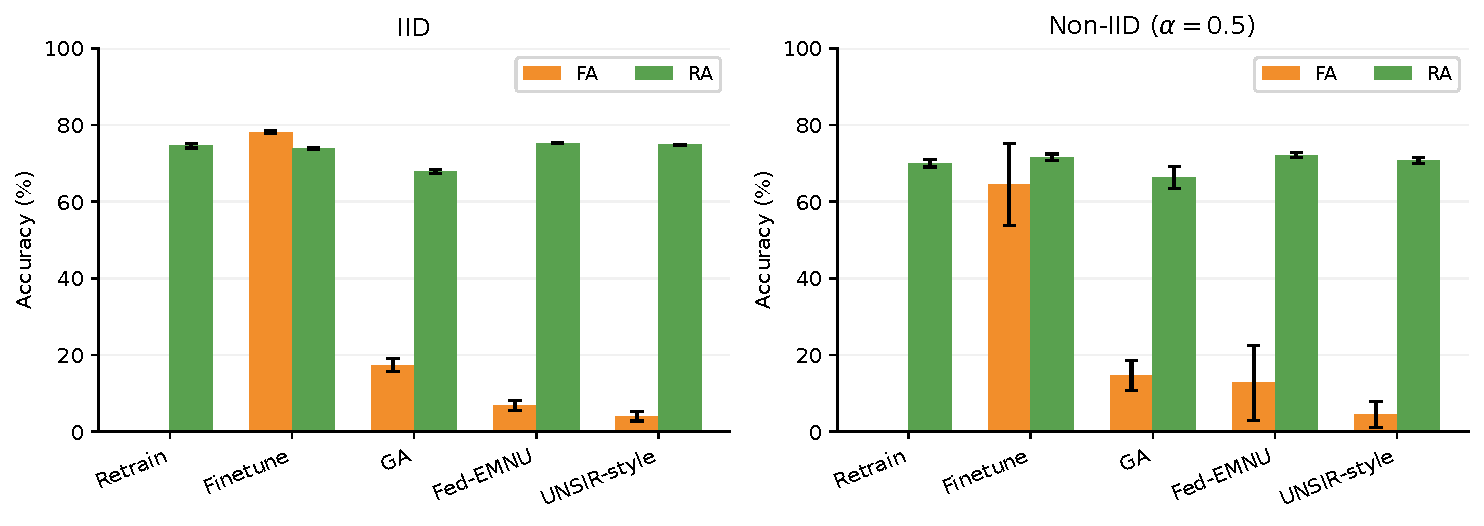
\includegraphics[width=\linewidth]{additional_effectiveness.pdf}
\caption{Primary-method target-class accuracy (FA) and retained accuracy (RA). Bars and whiskers are mean and sample SD across five seeds, using the same summaries as Tables~\ref{tab:iid-utility} and~\ref{tab:noniid-utility}. Lower FA indicates class suppression, not a deletion guarantee.}
\label{fig:additional-effectiveness}\end{figure}

\subsection{Unlearning Efficiency}
\label{sec:efficiency}
The paired Retrain/Fed-EMNU method-time ratio is $21.54\pm0.35$ under IID
and $19.56\pm0.71$ under Non-IID. The corresponding UNSIR-style/Fed-EMNU
ratios are $0.60\pm0.08$ and $0.55\pm0.03$, and GA/Fed-EMNU is
$0.14\pm0.01$ and $0.14\pm0.03$. A ratio below one means the named baseline
is faster. Finetune/Fed-EMNU ratios are $1.03\pm0.04$ and $1.06\pm0.16$.
These are paired compute/serialization ratios; evaluation and real transport
are excluded. Non-IID seed 45 took 114.20 s for Fed-EMNU, whereas the other
events took approximately 21--23 s. Its cause is unresolved and it is retained
in the reported mean and SD. The event carries 868.83 MiB of tensor payload
on average in both partitions; faster computation is not a network guarantee.

Figure~\ref{fig:additional-efficiency} shows the measured costs and variability.

\begin{figure}[htbp]\centering
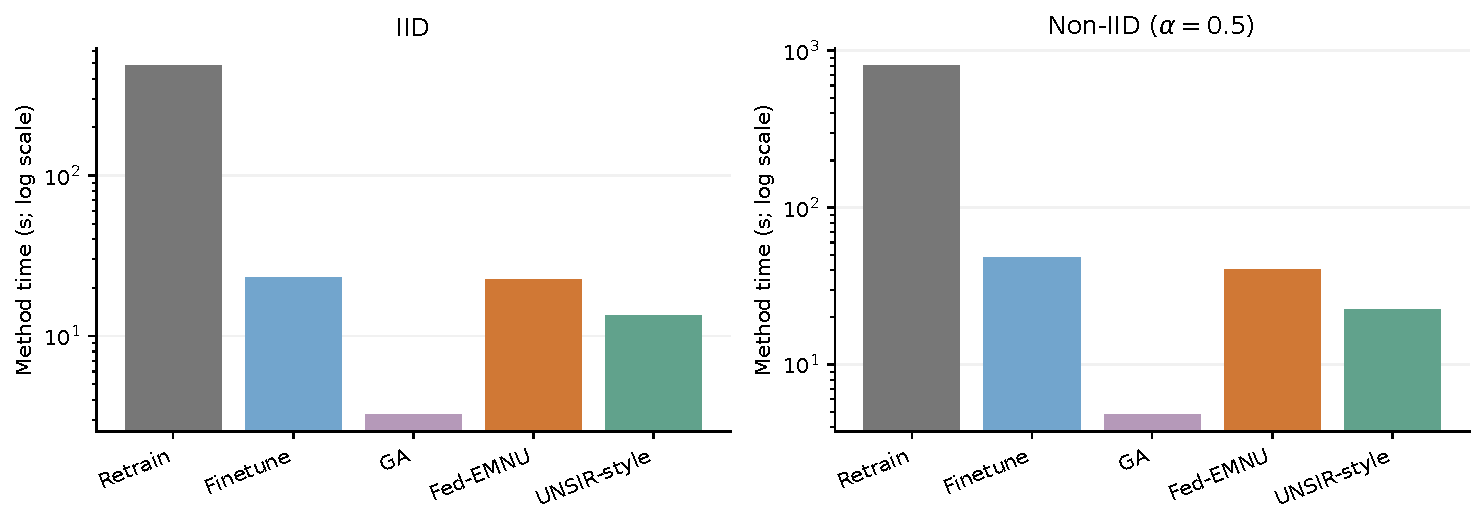
\includegraphics[width=\linewidth]{additional_efficiency.pdf}
\caption{Primary method time, arithmetic mean across five seeds. Sample SD is reported in the main utility tables; it is omitted here because the Non-IID retraining SD exceeds its mean and a logarithmic error interval would cross zero. A logarithmic axis displays fast update methods and retained-data retraining together. Timing includes local computation and serialization, and excludes evaluation and real transport. The unresolved Non-IID timing outlier is retained.}
\label{fig:additional-efficiency}\end{figure}

\subsection{Ablation of Unlearning and Enhancement}
\label{sec:ablation}
To explain how the existing components contribute, Figure~\ref{fig:ablation}
compares the full workflow with unlearning alone (impair-only) and enhancement
alone (repair-only), using the same request checkpoints across five seeds.
These controls remove one existing stage and retain the prescribed budget of
the remaining stage; they introduce no additional component.

\textbf{Role of enhancement.} With unlearning alone, IID FA is
$1.92\pm1.29$\% but RA falls to $72.61\pm1.51$\%, compared with
$6.80\pm1.35$\% FA and $75.24\pm0.08$\% RA for the full workflow.
Under Non-IID, RA rises from $36.78\pm22.04$\% without enhancement to
$72.16\pm0.70$\% with both stages, while FA rises from $1.08\pm1.32$\%
to $12.70\pm9.68$\%. Enhancement therefore recovers retained utility in
this recipe, with some recovery of target-class predictions as well.

\textbf{Role of target-directed unlearning.} Enhancement alone preserves
RA ($75.56\pm0.33$\% IID; $72.82\pm0.76$\% Non-IID) but leaves FA at
$41.42\pm1.83$\% and $41.00\pm7.45$\%, respectively. Retained-only
enhancement is therefore insufficient to obtain the full workflow's target
suppression. Together, these controls support the complementary functions of
the two stages: target-directed updating supplies suppression, and enhancement
recovers retained-task utility. They explain the design's measured trade-off,
rather than establish that either primitive is new. Removing a stage also
reduces computation, so these are stage-removal controls, not equal-compute
comparisons or a proof of record deletion. They do not separately isolate
optimized noise from arbitrary synthetic inputs or other impair objectives.
\begin{figure}[htbp]\centering
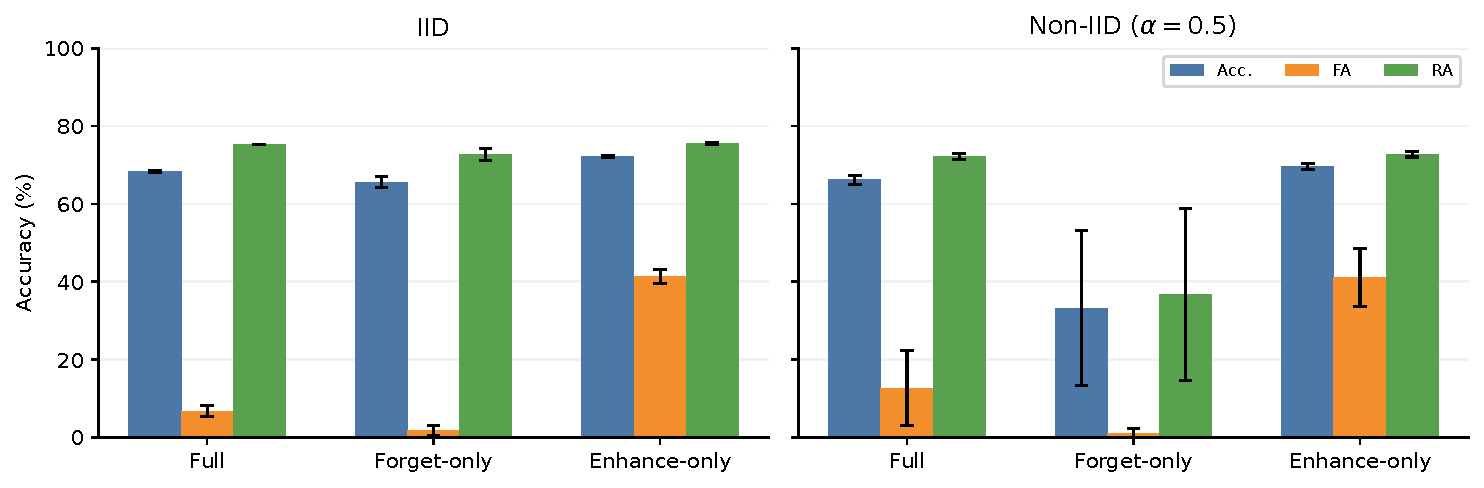
\includegraphics[width=\linewidth]{fig5_ablation_revised.pdf}
\caption{Two-stage ablation under IID and Non-IID partitions.
Bars show mean Acc., FA and RA; whiskers show sample SD across five seeds.
Forget-only denotes impair-only; Enhance-only denotes repair-only.
All controls use the same request checkpoints and retained-data references.}
\label{fig:ablation}\end{figure}

\subsection{Local Retained-Data Selection}
\label{sec:selection-results}
Figure~\ref{fig:filtering} compares random and confidence-based selection. Both controls use $rt=0.5$, identical per-class counts, and paired
checkpoints. Confidence minus random selection changes RA by
$-1.50\pm0.27$ percentage points under IID and $-0.84\pm0.61$ under Non-IID.
Their descriptive 95\% intervals are $[-1.837,-1.154]$ and
$[-1.592,-0.083]$ (Appendix~\ref{sec:uncertainty}). The evaluated recipe does
not support a confidence-selection advantage. These results do not establish an optimal retained ratio: the selection
comparison uses a single ratio, and the $rt=1$ main recipe is not a matched
ratio-only control for these experiments.
\begin{figure}[htbp]\centering
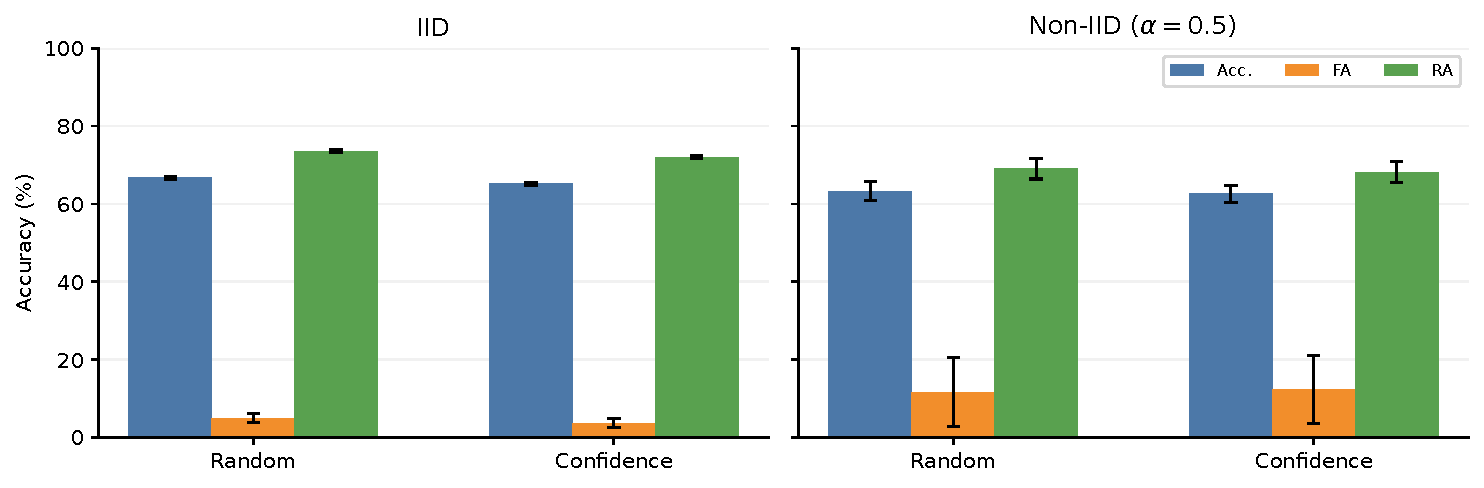
\includegraphics[width=\linewidth]{fig6_filtering_revised.pdf}
\caption{Matched retained-data selection at $rt=0.5$. Both partitions are evaluated. Bars and whiskers show mean and sample
SD across five paired seeds; metric colors match Figure~\ref{fig:ablation}.}
\label{fig:filtering}\end{figure}

\subsection{Random-Seed Variation}
\label{sec:seed-results}
Figure~\ref{fig:seed} shows mean and sample SD across five seeds in both partitions. Non-IID FA varies substantially ($12.70\pm9.68$\%),
although RA varies less ($72.16\pm0.70$\%). Variation is therefore not uniformly small across metrics and partitions. Primary confidence intervals and
reference-to-reference variation are reported in Appendices~\ref{sec:uncertainty}
and~\ref{sec:core-details}; small samples and variation in partition and schedule
limit general stability claims.
\begin{figure}[htbp]\centering
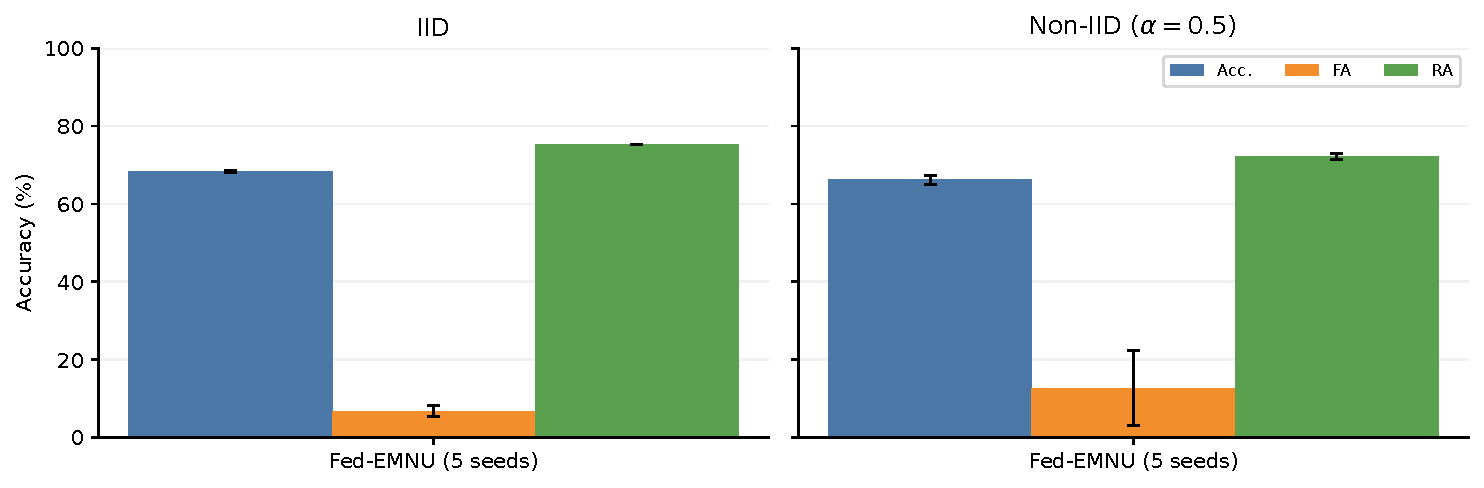
\includegraphics[width=\linewidth]{fig8_seed_revised.pdf}
\caption{Seed variation of the full method: mean $\pm$ sample SD across seeds
42--46. Both partitions are shown. Low FA alone is not a privacy or deletion
guarantee; the attack and reference diagnostics must be considered jointly.}
\label{fig:seed}\end{figure}

\subsection{Additional Evaluation}
\label{sec:extension-summary}
The complete additional studies are retained in Appendix~\ref{sec:extensions}.
ResNet34 extends the architecture evidence within the ResNet family. Stronger
heterogeneity ($\alpha=0.1$) exposes poor starting utility and sparse target
ownership, including the aggregation limitation in Section~\ref{sec:protocol}.
In CIFAR-100, FA remains $33.00\pm12.49$\% (IID) and $24.67\pm13.32$\%
(Non-IID), and target AUC exceeds the retraining reference; the fixed recipe
does not establish effective cross-dataset deletion.

The six PAR-code-based events use the same three-seed starting checkpoints as
their core comparators, with the adaptation described in
Appendix~\ref{sec:parprotocol}. PAR adaptation FA is $63.00\pm2.70$\% (IID)
and $54.23\pm5.81$\%; RA is $74.76\pm0.33$\% and $72.14\pm0.47$\%.
Its native budgets differ, and unavailable full-paper verification prevents
claiming an exact reproduction or refutation of the published method.

Twenty-client tests yield RA $71.41\pm0.80$\% (IID) and $66.69\pm1.41$\%
(Non-IID), with paired 20-minus-10-client RA differences of
$-3.88\pm0.84$ and $-5.46\pm0.58$ percentage points. Partitioning and local
batching also change, so this is a limited scale test. The two-request study
observes no class-0 rebound in six Fed-EMNU paths, with variable class-1
suppression. Five retained-only continuation rounds after the single-class
event also show no FA rebound in six paths, but target membership scores
remain different from the continued retained-data reference. Neither study
validates arbitrary request streams or future training. Full tables and
protocol boundaries remain available in the appendices.


\subsection{Controlled Comparisons and Robust Timing}
\label{sec:controlled-summary}
Matched objective controls use three paired seeds, common checkpoints, full
retained data and identical random ordering. At 80 noise steps/three repair
epochs, Fed-minus-UNSIR RA is $0.063\pm0.371$ percentage points under IID
and $-0.463\pm0.361$ under Non-IID; at 40 steps/one repair epoch it is
$-0.004\pm0.306$ and $-0.356\pm0.222$ points. These controls do not establish
a consistent advantage of the Fed-EMNU penalty. Optimized noise lowers target
attack AUC relative to Gaussian inputs by $0.029\pm0.012$ and
$0.022\pm0.018$, respectively, but has mixed accuracy effects.
Retained-count event weighting raises Non-IID RA by $0.896\pm0.224$ points
and FA by $0.600\pm0.557$ relative to equal weighting.

Separate comparisons impose common maximum compute/serialization caps of
10, 20, 30 and 40 seconds. All 48 events finish within their caps. Fed-EMNU
has higher mean RA at every cap, by 1.41/0.49/0.48/0.39 points under IID
and 4.50/1.81/1.29/1.56 points under Non-IID, but also higher FA and target
attack AUC throughout. These are time-capped adaptations with reported
realized steps and consumed times; early completion is not padded. The results
show a utility--suppression trade-off rather than dominance or a privacy gain.

Robust summaries retain the historical Non-IID timing outlier. Six technical
repeats reproduce the saved predictions exactly but do not reproduce its large
delay: seed 45 takes a median 25.76 seconds, versus 114.20 seconds originally.
The historical cause remains unresolved; repeats are not additional scientific
seeds. Appendix~\ref{sec:controlled-details} gives the full control protocols,
tables, timing distributions and limits, separately from the five-seed primary
comparison.

\subsection{Applicability and Failure Conditions}
\label{sec:applicability}
The fixed recipe should not be extrapolated beyond the evaluated conditions.
On CIFAR-100, target accuracy remains 33.00\% under IID and 24.67\% under
Non-IID, with target membership AUC above the matching references. The method
therefore fails to establish reliable class revocation on that dataset under
the stated recipe. At twenty clients, retained accuracy drops by 3.88 and 5.46
percentage points relative to paired ten-client runs. This does not support
a claim that utility is maintained as the federation grows. With stronger
heterogeneity, poor starting utility and sparse target ownership expose the
limits of updating only target holders; the current aggregation rule gives
other clients no separate repair contribution. ResNet34 adds depth within one
architecture family, without establishing architecture independence.

The mechanism is consequently an experimental option for approximate
class suppression in cooperative, available-client settings with similar
data and training conditions. Deployment would require representative local
validation of target behavior, retained utility, membership exposure and
resource use. The observed failures are part of the method's scope, not
exceptions removed from the evaluation. No universal operating threshold or
certified-deletion use case is established by this study.


\section{Conclusion}
\label{sec:conclusion}
The contribution is implementation-oriented: a specified federated adaptation
of existing impair--repair mechanisms and an empirical characterization of its
behavior. It establishes neither a new optimization principle nor general
superiority over UNSIR or PAR. Fed-EMNU integrates server-generated target-directed synthetic inputs,
client-local retained-data control and coordinated unlearning--enhancement
updates into a federated class-unlearning workflow. The formulation specifies
request scope, synthetic labels, local budgets and server aggregation.
The five-seed component-removal experiments explain the design: unlearning
supplies target suppression, while enhancement recovers retained-task utility.
Under Non-IID partitions, enhancement raises mean RA from $36.78$\% to
$72.16$\%; enhancement alone leaves mean FA at $41.00$\%, compared with
$12.70$\% for the full workflow. These findings support complementary stage
roles and quantify the associated suppression--utility trade-off.

The reference-based evaluation measures this trade-off together with runtime
and membership behavior. Fed-EMNU has higher mean retained accuracy than the
UNSIR-style adaptation in the primary settings, while that comparator is faster
and yields lower target accuracy. Matched subset controls do not support a
confidence-ranking advantage. The additional matched-update-budget objective controls
do not show a consistent advantage of the Fed-EMNU norm penalty. Optimized
noise lowers target attack AUC relative to Gaussian inputs but has mixed
accuracy effects across partitions. Non-IID event weighting
increases retained utility with some increase in residual target accuracy.
Comparisons under common maximum time caps likewise show retained-utility gains accompanied
by higher residual target accuracy and attack AUC. These findings restrict the scientific contribution to a specified adaptation
and empirical characterization rather than a demonstrated superior mechanism.
Dataset, architecture, heterogeneity,
twenty-client, two-request and retained-only continuation studies extend the
evaluation beyond the primary setting.

\textbf{Limitations and future work.} The method provides approximate class
suppression: behavioral and membership differences from retraining remain,
and CIFAR-100 retains substantial target accuracy and attack AUC above its
reference. The protocol assumes cooperative, available affected clients;
target-holder-only aggregation gives unaffected clients no separate repair
update under sparse ownership. Requester-level effectiveness, unavailable
clients, arbitrary request streams and unrestricted future training remain
open. The evaluated scope is two CIFAR datasets, one ResNet family and
ten/twenty simulated clients, with five primary and three extension seeds.
One loss-based attack does not certify deletion or exhaust privacy threats.
Stage removal changes compute. Additional within-budget objective and
event-weight controls address some confounding, but do not isolate every
interaction or establish superiority at equal wall-clock latency. The PAR comparison is
limited to the code-based adaptation documented in Appendix~\ref{sec:parprotocol}.
Future work should examine broader client participation in repair,
alternative local selection criteria and longer request sequences.
Resource-constrained edge deployments also require joint measurement of client
energy, memory, actual uplink/downlink latency and request completion time.
Salman et al.~\cite{ref26} study a hybrid content delivery network (CDN)
architecture combining edge caching, multi-access edge computing (MEC)
offloading and Q-learning-based adaptive routing. That work provides an
application context for future investigations of where unlearning computations
should execute under varying resource availability; it does not evaluate
Fed-EMNU or establish its communication efficiency. Any offloading design must
also specify the changed data-access and trust assumptions.
\vspace{10pt}
\noindent\textbf{Author Contributions:} Conceptualization, Jiale Wang and
Jianhua Wang; methodology, Jiale Wang; software, Jiale Wang; validation, Jiale
Wang, Zixiao Liu and Jianhua Wang; formal analysis, Jiale Wang; investigation,
Jiale Wang; data curation, Jiale Wang; writing--original draft preparation,
Jiale Wang; writing--review and editing, Jiale Wang, Zixiao Liu and Jianhua
Wang; visualization, Jiale Wang; supervision, Jianhua Wang; project
administration, Jianhua Wang; funding acquisition, Jianhua Wang.
\vspace{6pt}
\noindent\textbf{Funding:} This research was funded by the Central
Government-Guided Local Science and Technology Development Fund
(No. YDZJSX2025D029).
\vspace{6pt}
\noindent\textbf{Conflicts of Interest:} The authors declare no conflict of interest.
\vspace{6pt}
\noindent\textbf{Data and Code Availability:} CIFAR-10 and CIFAR-100 are publicly available
from their original dataset page, \url{https://www.cs.toronto.edu/~kriz/cifar.html}.
The original implementation repository is
\url{https://github.com/Daoge12/Fed-EMNU}. The revision branch at
\url{https://github.com/Daoge12/Fed-EMNU/tree/codex/revision-2026-11}
provides the manuscript source, frozen runner/adapter snapshots, protocols,
per-event configurations and numerical metrics for all 412 formal recorded
stages/events, seed-level control summaries, and a dependency-aware replay
catalog. The revision README gives environment setup, dataset preparation,
suite-to-experiment mapping, dry-run commands and a separate, permanently
excluded small pipeline check. The original experimental source snapshot is
\texttt{8fa5b727b820eac8c69a8c85e83840ba1951904d}; later commits improve
documentation and packaging. Public summary checks validate record coverage,
source hashes and agreement with the released seed-level control summaries.
They do not rerun model training or independently reconstruct membership attacks.
Full saved prediction arrays, raw execution logs, CIFAR data and checkpoint
weights are excluded. Replay commands regenerate those outputs; floating-point
results and actual execution times may vary across environments. In particular,
time-capped stopping is hardware dependent. Exact historical original-result
provenance remains unresolved.

\clearpage
\appendixstart
\appendix
\section{Detailed Primary Diagnostics}
\label{sec:core-details}
\noindent\textbf{Reading the appendix tables.}
FA is target-class accuracy and RA is retained-class accuracy, both in percent;
pp denotes percentage points. Target AUC is the declared target membership
attack AUC, and TV is mean total-variation distance from the stated retained-data
reference, both in probability units. Exec. denotes measured execution seconds
over the declared timing boundary, not an update budget or time cap. Unless a
caption specifies otherwise, entries are mean $\pm$ sample standard deviation;
Appendix A uses five seeds and extension/control tables use three paired seeds.
Technical timing repetitions and quartile summaries are labeled separately.
``---'' means not applicable or unavailable, never zero. UNSIR in the objective
control row names denotes the UNSIR-style federated objective adaptation.
\par

These tables supplement the five-seed main comparison. Values are mean $\pm$
sample SD; the identical checkpoints, references and attack splits are used.
\begin{table}[H]\centering\small
\caption{IID reference distance and class-conditioned attack. AUC and advantage are target-class values.}
\label{tab:iid-distance}
\begin{tabular}{lrrrr}\toprule Method & Disagree (\%) & TV & Target AUC & Target advantage\\\midrule
Retrain & $0.00 \pm 0.00$ & $0.000 \pm 0.000$ & $0.508 \pm 0.026$ & $0.010 \pm 0.036$\\
Finetune & $31.10 \pm 0.56$ & $0.309 \pm 0.004$ & $0.656 \pm 0.008$ & $0.284 \pm 0.015$\\
GA & $34.11 \pm 1.41$ & $0.341 \pm 0.013$ & $0.615 \pm 0.002$ & $0.182 \pm 0.028$\\
Fed-EMNU & $25.58 \pm 0.32$ & $0.254 \pm 0.003$ & $0.620 \pm 0.017$ & $0.177 \pm 0.030$\\
UNSIR-style & $25.86 \pm 0.48$ & $0.259 \pm 0.005$ & $0.606 \pm 0.023$ & $0.157 \pm 0.044$\\
\bottomrule\end{tabular}\end{table}

\begin{table}[H]\centering\small
\caption{IID retained-class attack and attack differences from Retrain. Differences use identical member/nonmember indices and separately calibrated model-specific thresholds.}
\label{tab:iid-attack}
\begin{tabular}{lrrrr}\toprule Method & Retained AUC & Retained adv. & $\Delta$ target AUC & $\Delta$ retained AUC\\\midrule
Retrain & $0.674 \pm 0.005$ & $0.322 \pm 0.010$ & 0 (self) & 0 (self)\\
Finetune & $0.680 \pm 0.002$ & $0.337 \pm 0.010$ & $0.147 \pm 0.027$ & $0.006 \pm 0.004$\\
GA & $0.632 \pm 0.001$ & $0.223 \pm 0.004$ & $0.106 \pm 0.027$ & $-0.042 \pm 0.006$\\
Fed-EMNU & $0.640 \pm 0.005$ & $0.250 \pm 0.014$ & $0.111 \pm 0.039$ & $-0.034 \pm 0.005$\\
UNSIR-style & $0.635 \pm 0.007$ & $0.239 \pm 0.018$ & $0.098 \pm 0.039$ & $-0.038 \pm 0.008$\\
\bottomrule\end{tabular}\end{table}

\begin{table}[H]\centering\small
\caption{IID matched selection and stage controls. All values use the same reference and pretrained states as the main comparison.}
\label{tab:iid-controls}
\begin{tabular}{lrrrr}\toprule Control & FA (\%) & RA (\%) & TV & Exec. (s)\\\midrule
Random (rt=0.5) & $4.96 \pm 1.18$ & $73.53 \pm 0.34$ & $0.272 \pm 0.005$ & $13.03 \pm 3.13$\\
Confidence (rt=0.5) & $3.72 \pm 1.19$ & $72.03 \pm 0.38$ & $0.281 \pm 0.005$ & $14.18 \pm 3.36$\\
Impair only & $1.92 \pm 1.29$ & $72.61 \pm 1.51$ & $0.301 \pm 0.023$ & $8.36 \pm 1.87$\\
Repair only & $41.42 \pm 1.83$ & $75.56 \pm 0.33$ & $0.271 \pm 0.004$ & $14.60 \pm 2.74$\\
\bottomrule\end{tabular}\end{table}

\begin{table}[H]\centering\small
\caption{Non-IID ($\alpha=0.5$) reference distance and class-conditioned attack. AUC and advantage are target-class values.}
\label{tab:noniid-distance}
\begin{tabular}{lrrrr}\toprule Method & Disagree (\%) & TV & Target AUC & Target advantage\\\midrule
Retrain & $0.00 \pm 0.00$ & $0.000 \pm 0.000$ & $0.487 \pm 0.033$ & $-0.021 \pm 0.050$\\
Finetune & $34.04 \pm 1.21$ & $0.337 \pm 0.011$ & $0.641 \pm 0.017$ & $0.221 \pm 0.027$\\
GA & $35.57 \pm 1.78$ & $0.354 \pm 0.017$ & $0.617 \pm 0.015$ & $0.178 \pm 0.041$\\
Fed-EMNU & $31.69 \pm 0.92$ & $0.313 \pm 0.008$ & $0.596 \pm 0.006$ & $0.144 \pm 0.024$\\
UNSIR-style & $32.35 \pm 1.19$ & $0.325 \pm 0.012$ & $0.578 \pm 0.008$ & $0.115 \pm 0.010$\\
\bottomrule\end{tabular}\end{table}

\begin{table}[H]\centering\small
\caption{Non-IID ($\alpha=0.5$) retained-class attack and attack differences from Retrain. Differences use identical member/nonmember indices and separately calibrated model-specific thresholds.}
\label{tab:noniid-attack}
\begin{tabular}{lrrrr}\toprule Method & Retained AUC & Retained adv. & $\Delta$ target AUC & $\Delta$ retained AUC\\\midrule
Retrain & $0.640 \pm 0.010$ & $0.235 \pm 0.019$ & 0 (self) & 0 (self)\\
Finetune & $0.655 \pm 0.005$ & $0.261 \pm 0.010$ & $0.154 \pm 0.024$ & $0.015 \pm 0.010$\\
GA & $0.625 \pm 0.006$ & $0.202 \pm 0.018$ & $0.130 \pm 0.026$ & $-0.014 \pm 0.008$\\
Fed-EMNU & $0.624 \pm 0.009$ & $0.210 \pm 0.017$ & $0.110 \pm 0.039$ & $-0.016 \pm 0.016$\\
UNSIR-style & $0.609 \pm 0.012$ & $0.182 \pm 0.020$ & $0.091 \pm 0.033$ & $-0.031 \pm 0.013$\\
\bottomrule\end{tabular}\end{table}

\begin{table}[H]\centering\small
\caption{Non-IID ($\alpha=0.5$) matched selection and stage controls. All values use the same reference and pretrained states as the main comparison.}
\label{tab:noniid-controls}
\begin{tabular}{lrrrr}\toprule Control & FA (\%) & RA (\%) & TV & Exec. (s)\\\midrule
Random (rt=0.5) & $11.68 \pm 8.85$ & $69.00 \pm 2.60$ & $0.341 \pm 0.013$ & $26.05 \pm 32.16$\\
Confidence (rt=0.5) & $12.40 \pm 8.72$ & $68.16 \pm 2.73$ & $0.346 \pm 0.011$ & $24.09 \pm 25.16$\\
Impair only & $1.08 \pm 1.32$ & $36.78 \pm 22.04$ & $0.680 \pm 0.169$ & $9.20 \pm 1.00$\\
Repair only & $41.00 \pm 7.45$ & $72.82 \pm 0.76$ & $0.325 \pm 0.014$ & $13.94 \pm 0.12$\\
\bottomrule\end{tabular}\end{table}
\paragraph{Variation among retraining references.}

For IID, pairwise TV among the five retained-data references ranged from 0.247 to 0.259, and prediction disagreement ranged from 24.95\% to 26.19\%. These comparisons share the same retained global records and test set but vary initialization, client partition and schedule together. The ten pairs are dependent and are reported only as descriptive context, not as additional independent runs or a certified tolerance for unlearning.
For Non-IID, pairwise TV among the five retained-data references ranged from 0.317 to 0.349, and prediction disagreement ranged from 32.34\% to 35.40\%. These comparisons share the same retained global records and test set but vary initialization, client partition and schedule together. The ten pairs are dependent and are reported only as descriptive context, not as additional independent runs or a certified tolerance for unlearning.

\begin{figure}[htbp]\centering
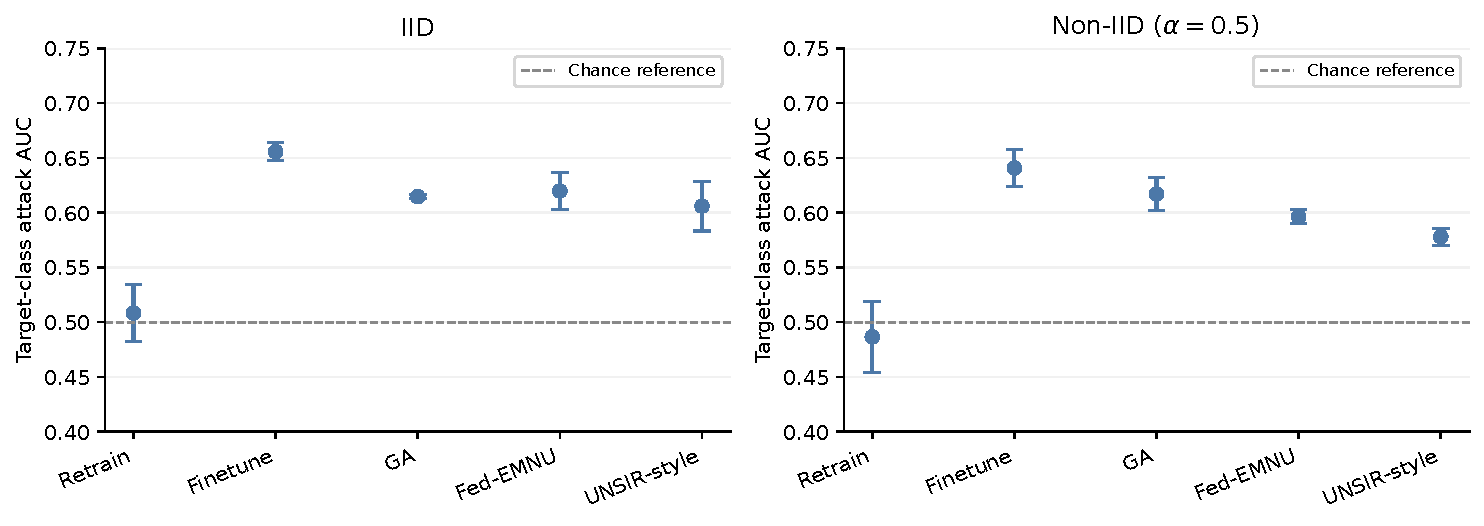
\includegraphics[width=\linewidth]{additional_privacy.pdf}
\caption{Target-class loss-based membership-inference AUC for the five primary methods, mean $\pm$ sample SD across five seeds. The dashed 0.5 line denotes chance reference for this attack, not a privacy or deletion threshold. AUC is interpreted against retained-data retraining.}
\label{fig:additional-privacy}\end{figure}

\section{PAR Code-Based Comparison Protocol}
\label{sec:parprotocol}
The PAR adaptation loads each of the six original CIFAR-10/ResNet18 checkpoints
and its matching retained-data reference. It retains our $32\times32$ real-image
preprocessing and normalization to share exact starting weights. Public PAR
code instead resizes real CIFAR examples to $128\times128$ with its own
normalization. This is a material adaptation; published numbers are not reused.

Following the inspected source, a generator maps 128-dimensional Gaussian
latents through a 128-channel $8\times8$ stem, two upsampling stages and
three-channel Conv/BatchNorm output. Adam at 0.001 minimizes negative target CE
plus 0.01 times the mean per-image squared L2 norm, for five groups of eight
updates. Each group reuses its latent batch. ReduceLROnPlateau (factor 0.5,
patience 2) receives the final loss of each group. The request model is frozen
in evaluation mode. Eight synthetic batches are extracted in generator training
mode using a single new latent batch, with target labels and no clipping.

Every client performs one impair epoch on local retained plus synthetic
examples, followed by equal aggregation; ten rounds then each perform one
retained-data epoch at every client and equal aggregation. Local Adam uses
0.001 and resets on each call. Floating states use equal weights, while integer
BN counters use max for compatibility with the canonical evaluator. We use the
fixed final repair round; the public code's retained-test best-checkpoint
selection is not used. Timing additionally includes generator/provenance
serialization and excludes post-hoc evaluation. Native budgets are preserved
and reported, rather than interpreted as an equal-compute comparison.
The frozen adapter, protocol and source hashes accompany each run. Full-paper
verification and exact published-protocol reproduction remain outstanding.


\section{Additional Experiments and Uncertainty}
\label{sec:extensions}
The following complete evidence is retained, including unfavorable outcomes.
Extension studies use three seeds; primary uncertainty intervals use five.
\subsection{Completed Follow-Up Experiments}

\label{sec:followup}

The follow-up retains the fixed training recipe and three seeds (42--44). It adds 36 CIFAR-10/ResNet34 stages (six methods in each partition), 30 ResNet18 stages at Dirichlet $\alpha=0.1$ (including controls), and six PAR-code-based events on the original core checkpoints. These extensions do not replace or tune the core results.  Values below are mean $\pm$ sample SD, $n=3$. The PAR comparison uses three-seed core comparators; CIFAR-100 results are in Appendix~\ref{sec:cifar100} and the twenty-client extension is in Appendix~\ref{sec:clients20}.

\begin{table}[H]
\caption{ResNet34 architecture extension on CIFAR-10 (IID). TV is against the corresponding ResNet34 retained-data reference.}
\label{tab:r34-iid}
\centering\footnotesize\setlength{\tabcolsep}{3.5pt}
\begin{tabular}{lrrrrr}
\toprule
Method & FA (\%) & RA (\%) & Target AUC & TV & Exec. (s)\\
\midrule
Original & $77.17 \pm 1.93$ & $73.00 \pm 0.28$ & $0.643 \pm 0.010$ & --- & $1185.13 \pm 159.23$\\
Retrain & $0.00 \pm 0.00$ & $74.48 \pm 0.06$ & $0.511 \pm 0.016$ & $0.000 \pm 0.000$ & $1073.87 \pm 146.93$\\
Finetune & $73.13 \pm 0.38$ & $73.12 \pm 0.25$ & $0.651 \pm 0.018$ & $0.312 \pm 0.005$ & $57.84 \pm 1.15$\\
GA & $14.20 \pm 1.49$ & $67.70 \pm 0.67$ & $0.603 \pm 0.011$ & $0.341 \pm 0.006$ & $7.79 \pm 0.14$\\
Fed-EMNU & $5.40 \pm 0.82$ & $74.67 \pm 0.61$ & $0.600 \pm 0.018$ & $0.261 \pm 0.002$ & $54.51 \pm 0.38$\\
UNSIR-style & $2.27 \pm 0.42$ & $74.06 \pm 0.65$ & $0.592 \pm 0.015$ & $0.262 \pm 0.007$ & $31.02 \pm 0.31$\\
\bottomrule
\end{tabular}
\end{table}

\begin{table}[H]
\caption{ResNet34 architecture extension on CIFAR-10 (Non-IID, $\alpha=0.5$). TV is against the corresponding ResNet34 retained-data reference.}
\label{tab:r34-noniid}
\centering\footnotesize\setlength{\tabcolsep}{3.5pt}
\begin{tabular}{lrrrrr}
\toprule
Method & FA (\%) & RA (\%) & Target AUC & TV & Exec. (s)\\
\midrule
Original & $69.63 \pm 10.59$ & $68.93 \pm 0.72$ & $0.625 \pm 0.005$ & --- & $911.10 \pm 149.88$\\
Retrain & $0.00 \pm 0.00$ & $69.20 \pm 0.64$ & $0.505 \pm 0.026$ & $0.000 \pm 0.000$ & $762.58 \pm 10.36$\\
Finetune & $68.97 \pm 7.60$ & $71.20 \pm 0.66$ & $0.641 \pm 0.006$ & $0.344 \pm 0.003$ & $37.90 \pm 0.63$\\
GA & $14.90 \pm 5.26$ & $63.60 \pm 1.84$ & $0.605 \pm 0.005$ & $0.366 \pm 0.015$ & $5.67 \pm 0.22$\\
Fed-EMNU & $8.67 \pm 1.36$ & $72.39 \pm 1.37$ & $0.609 \pm 0.017$ & $0.310 \pm 0.017$ & $37.29 \pm 0.50$\\
UNSIR-style & $10.10 \pm 7.01$ & $70.94 \pm 1.03$ & $0.595 \pm 0.021$ & $0.333 \pm 0.016$ & $19.96 \pm 0.62$\\
\bottomrule
\end{tabular}
\end{table}

This within-family architecture extension does not establish architecture independence. The same fixed recipe is evaluated without test-based retuning; its utility, forgetting and attack values must be considered jointly.

\begin{table}[H]
\caption{Stronger heterogeneity on CIFAR-10/ResNet18 ($\alpha=0.1$). Low initial utility limits the interpretation of low final FA.}
\label{tab:alpha01}
\centering\footnotesize\setlength{\tabcolsep}{3.5pt}
\begin{tabular}{lrrrrr}
\toprule
Method & FA (\%) & RA (\%) & Target AUC & TV & Exec. (s)\\
\midrule
Original & $42.67 \pm 40.93$ & $40.57 \pm 7.79$ & $0.591 \pm 0.039$ & --- & $503.77 \pm 7.23$\\
Retrain & $0.00 \pm 0.00$ & $39.38 \pm 11.81$ & $0.492 \pm 0.014$ & $0.000 \pm 0.000$ & $459.88 \pm 9.79$\\
Finetune & $47.87 \pm 34.35$ & $49.80 \pm 3.17$ & $0.592 \pm 0.029$ & $0.463 \pm 0.032$ & $11.86 \pm 3.78$\\
GA & $10.30 \pm 17.32$ & $39.89 \pm 6.67$ & $0.558 \pm 0.044$ & $0.383 \pm 0.072$ & $3.08 \pm 0.21$\\
Fed-EMNU & $1.87 \pm 2.31$ & $40.81 \pm 11.25$ & $0.547 \pm 0.010$ & $0.597 \pm 0.114$ & $11.63 \pm 3.80$\\
UNSIR-style & $3.70 \pm 5.15$ & $40.21 \pm 13.40$ & $0.561 \pm 0.019$ & $0.608 \pm 0.159$ & $6.51 \pm 1.91$\\
\bottomrule
\end{tabular}
\end{table}

At $\alpha=0.1$, Original RA is $40.57 \pm 7.79$\%, Retrain RA is $39.38 \pm 11.81$\%, and Fed-EMNU RA is $40.81 \pm 11.25$\%. Poor retained utility is therefore present before unlearning. Fed-EMNU target AUC is $0.547 \pm 0.010$, versus $0.492 \pm 0.014$ for Retrain. Confidence minus random RA at $rt=0.5$ is $-3.24 \pm 1.02$ percentage points and TV changes by $0.035 \pm 0.022$. These controls again provide no support for a confidence-ranking advantage.

The Fed-EMNU event includes 4, 5, 7 target-holding clients for seeds 42, 43 and 44, respectively. Replacing the global state with updates from only those clients can omit unaffected-client contributions. This is a protocol limitation under sparse target ownership; it is not evidence of robust heterogeneity handling.

\begin{table}[H]
\caption{PAR-code-based adaptation on the original three shared core ResNet18 checkpoints (IID). Native method budgets differ; this is not an equal-compute ablation.}
\label{tab:par-iid}
\centering\footnotesize\setlength{\tabcolsep}{3.5pt}
\begin{tabular}{lrrrrr}
\toprule
Method & FA (\%) & RA (\%) & Target AUC & TV & Exec. (s)\\
\midrule
Retrain & $0.00 \pm 0.00$ & $74.34 \pm 0.59$ & $0.515 \pm 0.015$ & $0.000 \pm 0.000$ & $428.59 \pm 2.64$\\
Fed-EMNU & $7.70 \pm 0.70$ & $75.29 \pm 0.05$ & $0.614 \pm 0.021$ & $0.255 \pm 0.003$ & $19.92 \pm 0.34$\\
UNSIR-style & $4.37 \pm 1.56$ & $74.79 \pm 0.19$ & $0.598 \pm 0.027$ & $0.262 \pm 0.005$ & $12.67 \pm 1.53$\\
PAR adaptation & $63.00 \pm 2.70$ & $74.76 \pm 0.33$ & $0.669 \pm 0.007$ & $0.295 \pm 0.003$ & $52.53 \pm 0.27$\\
\bottomrule
\end{tabular}
\end{table}

\begin{table}[H]
\caption{PAR-code-based adaptation on the original three shared core ResNet18 checkpoints (Non-IID, $\alpha=0.5$). Native method budgets differ; this is not an equal-compute ablation.}
\label{tab:par-noniid}
\centering\footnotesize\setlength{\tabcolsep}{3.5pt}
\begin{tabular}{lrrrrr}
\toprule
Method & FA (\%) & RA (\%) & Target AUC & TV & Exec. (s)\\
\midrule
Retrain & $0.00 \pm 0.00$ & $69.41 \pm 0.53$ & $0.478 \pm 0.024$ & $0.000 \pm 0.000$ & $424.14 \pm 3.79$\\
Fed-EMNU & $16.73 \pm 10.42$ & $72.15 \pm 0.94$ & $0.598 \pm 0.005$ & $0.316 \pm 0.006$ & $22.15 \pm 0.57$\\
UNSIR-style & $4.83 \pm 4.32$ & $70.63 \pm 1.07$ & $0.583 \pm 0.002$ & $0.329 \pm 0.013$ & $11.94 \pm 0.31$\\
PAR adaptation & $54.23 \pm 5.81$ & $72.14 \pm 0.47$ & $0.650 \pm 0.021$ & $0.343 \pm 0.007$ & $53.51 \pm 0.63$\\
\bottomrule
\end{tabular}
\end{table}

Under this code-based adaptation, PAR retains substantial target-class accuracy and its target MIA AUC remains above Retrain in both partitions. The ten repair rounds can restore utility and target behavior together; the experiment does not isolate that mechanism causally. These outcomes describe the specified shared-checkpoint adaptation, not a reproduction or refutation of the published PAR results.

PAR uses about $9.974$ GB of model and synthetic tensor payload per event (decimal units; transport framing excluded). It communicates one model download and upload per client at each of eleven aggregations. Its native multi-round budget, generator, learning rates, equal event aggregation and all-client participation differ jointly from Fed-EMNU. Paired comparisons record time, local optimizer steps and payload; observed differences cannot be assigned to one component.

\subsection{CIFAR-100 Dataset Extension}

\label{sec:cifar100}

CIFAR-100 uses ResNet18 with 100 output logits, ten clients, seeds 42--44, IID and Dirichlet $\alpha=0.5$, and global class 0 revocation. The same 50-round/five-local-epoch training recipe and fixed update budgets are used without dataset-specific test tuning. Each class provides 50 members and 50 nonmembers for calibration and the same counts on the disjoint attack test. Retained attack macros average 99 classes; target attacks concern class 0 alone. Values are mean $\pm$ sample SD across three seeds.

\begin{table}[H]
\caption{CIFAR-100/ResNet18 (IID), $n=3$. TV is against the corresponding retained-data reference.}
\label{tab:c100-iid}
\centering\footnotesize\setlength{\tabcolsep}{3.5pt}
\begin{tabular}{lrrrrr}
\toprule
Method & FA (\%) & RA (\%) & Target AUC & TV & Exec. (s)\\
\midrule
Original & $65.67 \pm 4.16$ & $35.39 \pm 0.81$ & $0.688 \pm 0.068$ & --- & $650.16 \pm 146.11$\\
Retrain & $0.00 \pm 0.00$ & $36.99 \pm 0.29$ & $0.515 \pm 0.026$ & $0.000 \pm 0.000$ & $677.85 \pm 52.04$\\
Finetune & $62.67 \pm 3.79$ & $36.61 \pm 0.64$ & $0.704 \pm 0.059$ & $0.621 \pm 0.006$ & $35.72 \pm 0.43$\\
GA & $31.67 \pm 4.04$ & $32.14 \pm 0.58$ & $0.640 \pm 0.045$ & $0.661 \pm 0.009$ & $1.81 \pm 0.04$\\
Fed-EMNU & $33.00 \pm 12.49$ & $35.79 \pm 0.71$ & $0.712 \pm 0.076$ & $0.621 \pm 0.008$ & $34.34 \pm 0.52$\\
UNSIR-style & $23.33 \pm 13.05$ & $33.05 \pm 0.70$ & $0.680 \pm 0.070$ & $0.656 \pm 0.013$ & $19.79 \pm 0.15$\\
\bottomrule
\end{tabular}
\end{table}

Under IID, Original RA is $35.39 \pm 0.81$\%, Retrain RA is $36.99 \pm 0.29$\%, and Fed-EMNU RA is $35.79 \pm 0.71$\%. Fed-EMNU FA is $33.00 \pm 12.49$\%; target AUC is $0.712 \pm 0.076$ versus $0.515 \pm 0.026$ for Retrain. These results are interpreted against the dataset-specific initial utility and reference, rather than treating low FA alone as evidence of deletion or robustness.

\begin{table}[H]
\caption{CIFAR-100/ResNet18 (Non-IID, $\alpha=0.5$), $n=3$. TV is against the corresponding retained-data reference.}
\label{tab:c100-noniid}
\centering\footnotesize\setlength{\tabcolsep}{3.5pt}
\begin{tabular}{lrrrrr}
\toprule
Method & FA (\%) & RA (\%) & Target AUC & TV & Exec. (s)\\
\midrule
Original & $64.67 \pm 8.39$ & $34.55 \pm 0.99$ & $0.643 \pm 0.043$ & --- & $629.51 \pm 137.29$\\
Retrain & $0.00 \pm 0.00$ & $34.56 \pm 1.04$ & $0.425 \pm 0.020$ & $0.000 \pm 0.000$ & $593.40 \pm 122.62$\\
Finetune & $60.67 \pm 9.24$ & $35.86 \pm 0.74$ & $0.673 \pm 0.031$ & $0.628 \pm 0.006$ & $25.61 \pm 8.66$\\
GA & $24.00 \pm 9.00$ & $30.72 \pm 1.78$ & $0.627 \pm 0.049$ & $0.660 \pm 0.011$ & $1.58 \pm 0.57$\\
Fed-EMNU & $24.67 \pm 13.32$ & $34.13 \pm 0.90$ & $0.640 \pm 0.071$ & $0.641 \pm 0.015$ & $28.83 \pm 8.19$\\
UNSIR-style & $21.67 \pm 10.02$ & $32.62 \pm 0.92$ & $0.586 \pm 0.049$ & $0.658 \pm 0.010$ & $16.68 \pm 3.85$\\
\bottomrule
\end{tabular}
\end{table}

Under Non-IID, Original RA is $34.55 \pm 0.99$\%, Retrain RA is $34.56 \pm 1.04$\%, and Fed-EMNU RA is $34.13 \pm 0.90$\%. Fed-EMNU FA is $24.67 \pm 13.32$\%; target AUC is $0.640 \pm 0.071$ versus $0.425 \pm 0.020$ for Retrain. These results are interpreted against the dataset-specific initial utility and reference, rather than treating low FA alone as evidence of deletion or robustness.

\subsection{Five-Seed Uncertainty Analysis}

\label{sec:uncertainty}

The primary CIFAR-10/ResNet18 study uses five independent seeds (42--46) with matching protocols and budgets. The main utility tables and Appendix~\ref{sec:core-details} diagnostics use all five seeds. Two-sided 95\% Student-$t$ intervals use $\bar{x}\pm t_{0.975,4}s/\sqrt{5}$, assuming independent approximately normal seed-level measurements or paired differences. Intervals are unadjusted descriptive summaries across many metrics; they are not simultaneous guarantees, equivalence tests or privacy bounds. We do not clip endpoints to the metric range. Five seeds remain limited.

\begin{table}[H]\centering\small

\caption{Primary Fed-EMNU mean and descriptive 95\% intervals, five seeds. FA/RA use percent; AUC and TV use probability units.}

\label{tab:five-ci}

\begin{tabular}{llrr}\toprule Setting & Metric & Mean & 95\% interval\\\midrule

IID & FA & 6.800 & $[5.123, 8.477]$\\

IID & RA & 75.244 & $[75.145, 75.343]$\\

IID & Target AUC & 0.620 & $[0.599, 0.641]$\\

IID & TV & 0.254 & $[0.251, 0.258]$\\

Non-IID & FA & 12.700 & $[0.675, 24.725]$\\

Non-IID & RA & 72.164 & $[71.295, 73.034]$\\

Non-IID & Target AUC & 0.596 & $[0.588, 0.604]$\\

Non-IID & TV & 0.313 & $[0.303, 0.324]$\\

\bottomrule\end{tabular}\end{table}

IID confidence minus random selection has RA difference $-1.50$ percentage points (95\% interval $[-1.837, -1.154]$) and TV difference $0.009$ (interval $[0.006, 0.012]$). These are checkpoint-paired comparisons with identical per-class selected counts. They do not support a general confidence-selection advantage.

Non-IID confidence minus random selection has RA difference $-0.84$ percentage points (95\% interval $[-1.592, -0.083]$) and TV difference $0.005$ (interval $[-0.004, 0.015]$). These are checkpoint-paired comparisons with identical per-class selected counts. They do not support a general confidence-selection advantage.

\subsection{Multiple Targets and Two Sequential Requests}

\label{sec:sequence}

This follow-up evaluates simultaneous revocation of classes $\{0,1\}$ and sequential revocation $\{0\}\rightarrow\{1\}$ on CIFAR-10/ResNet18, ten clients, IID and $\alpha=0.5$, seeds 42--44.

Each sequential method uses its own class-0 core output as the next parent; second-event initial states therefore differ across methods. Current request labels control synthetic inputs, GA access and target-holder participation; cumulative labels control quarantine, reference and evaluation. Both paths exclude classes 0 and 1 from retained repair. All final outputs use the same seed-specific, freshly initialized 50-round reference trained without both classes. Its original partition and client schedule are retained. Historical member/attack splits are identical across paths, with target macros over two classes and retained macros over eight. Total sequential cost includes the first and second events; the paths have different native budgets and are not an equal-compute ablation. Values are mean $\pm$ sample SD, $n=3$.

\begin{table}[H]\centering\footnotesize\setlength{\tabcolsep}{3pt}

\caption{IID two-target final behavior and total event time, three seeds. Sim. is simultaneous; Seq. includes both requests.}

\label{tab:sequence-iid}

\begin{tabular}{llrrrrr}\toprule Method & Path & FA (\%) & RA (\%) & Target AUC & TV & Total exec. (s)\\\midrule

Finetune & Sim. & $81.10 \pm 0.57$ & $72.58 \pm 0.34$ & $0.638 \pm 0.007$ & $0.387 \pm 0.002$ & $38.67 \pm 28.32$\\

Finetune & Seq. & $79.40 \pm 0.91$ & $73.02 \pm 0.28$ & $0.642 \pm 0.006$ & $0.382 \pm 0.002$ & $55.01 \pm 22.02$\\

GA & Sim. & $15.80 \pm 2.63$ & $65.93 \pm 0.98$ & $0.584 \pm 0.018$ & $0.393 \pm 0.015$ & $6.89 \pm 1.81$\\

GA & Seq. & $35.97 \pm 2.70$ & $67.45 \pm 1.07$ & $0.597 \pm 0.015$ & $0.395 \pm 0.015$ & $6.67 \pm 1.00$\\

Fed-EMNU & Sim. & $2.12 \pm 0.70$ & $75.02 \pm 0.41$ & $0.583 \pm 0.018$ & $0.255 \pm 0.006$ & $31.03 \pm 5.93$\\

Fed-EMNU & Seq. & $3.27 \pm 4.71$ & $75.72 \pm 0.21$ & $0.588 \pm 0.021$ & $0.251 \pm 0.009$ & $43.36 \pm 6.44$\\

UNSIR-style & Sim. & $1.73 \pm 0.36$ & $74.75 \pm 0.60$ & $0.573 \pm 0.015$ & $0.262 \pm 0.009$ & $22.77 \pm 5.22$\\

UNSIR-style & Seq. & $1.67 \pm 1.19$ & $74.63 \pm 0.16$ & $0.581 \pm 0.002$ & $0.259 \pm 0.000$ & $26.70 \pm 3.96$\\

\bottomrule\end{tabular}\end{table}

\begin{table}[H]\centering\footnotesize\setlength{\tabcolsep}{3pt}

\caption{Non-IID two-target final behavior and total event time, three seeds. Sim. is simultaneous; Seq. includes both requests.}

\label{tab:sequence-noniid}

\begin{tabular}{llrrrrr}\toprule Method & Path & FA (\%) & RA (\%) & Target AUC & TV & Total exec. (s)\\\midrule

Finetune & Sim. & $73.22 \pm 5.99$ & $69.53 \pm 1.28$ & $0.610 \pm 0.005$ & $0.414 \pm 0.017$ & $24.66 \pm 6.00$\\

Finetune & Seq. & $73.63 \pm 5.23$ & $70.09 \pm 0.92$ & $0.614 \pm 0.008$ & $0.420 \pm 0.009$ & $44.64 \pm 2.14$\\

GA & Sim. & $19.65 \pm 7.60$ & $63.20 \pm 3.14$ & $0.595 \pm 0.002$ & $0.402 \pm 0.023$ & $5.92 \pm 0.16$\\

GA & Seq. & $31.03 \pm 12.73$ & $64.25 \pm 3.65$ & $0.599 \pm 0.003$ & $0.416 \pm 0.014$ & $6.93 \pm 0.28$\\

Fed-EMNU & Sim. & $8.42 \pm 5.99$ & $72.00 \pm 0.54$ & $0.580 \pm 0.005$ & $0.320 \pm 0.008$ & $27.55 \pm 1.17$\\

Fed-EMNU & Seq. & $5.98 \pm 3.39$ & $72.70 \pm 0.20$ & $0.574 \pm 0.015$ & $0.310 \pm 0.010$ & $42.13 \pm 0.06$\\

UNSIR-style & Sim. & $7.65 \pm 4.55$ & $69.20 \pm 0.67$ & $0.563 \pm 0.009$ & $0.366 \pm 0.006$ & $17.37 \pm 0.62$\\

UNSIR-style & Seq. & $5.63 \pm 6.98$ & $71.61 \pm 0.64$ & $0.562 \pm 0.027$ & $0.323 \pm 0.014$ & $23.06 \pm 0.69$\\

\bottomrule\end{tabular}\end{table}

For Fed-EMNU, sequential final FA is $3.27 \pm 4.71$\% under IID and $5.98 \pm 3.39$\% under Non-IID. The corresponding RA is $75.72 \pm 0.21$\% and $72.70 \pm 0.20$\%. These cumulative averages must not hide an individual target that remains predictable. Class-specific posteriors and attacks are retained in each event artifact.

\begin{table}[H]\centering\small

\caption{Fed-EMNU class-specific FA after the second request. Change is class-0 FA after minus before event 2, in percentage points. Negative change indicates further suppression.}

\label{tab:sequence-rebound}

\begin{tabular}{lrrr}\toprule Setting & Class 0 FA (\%) & Class 1 FA (\%) & Class 0 change (pp)\\\midrule

IID & $0.03 \pm 0.06$ & $6.50 \pm 9.35$ & $-7.67 \pm 0.67$\\

Non-IID & $0.33 \pm 0.58$ & $11.63 \pm 6.33$ & $-16.40 \pm 9.85$\\

\bottomrule\end{tabular}\end{table}

None of the six Fed-EMNU paths shows increased class-0 test accuracy after the second event. However, class-1 final accuracy ranges from 1.0\% to 17.3\% under IID and from 4.7\% to 17.1\% under Non-IID; successful suppression of the earlier class therefore does not imply equally effective deletion of the new class. No federated continuation after the two-request outputs was evaluated. Appendix~\ref{sec:continuation} separately studies five retained-only rounds after a single class-0 request; neither study establishes absence of future relearning after an arbitrary request stream.

Fed-EMNU total tensor payload is 926,759,840 bytes for simultaneous revocation and 1,822,062,400 bytes for two sequential events. Local optimizer steps average 2000 versus 3120 under IID and 1988.33 versus 3098.67 under Non-IID. Extra sequential compute and two model exchanges per client must be considered with the utility differences. Actual transport delay and framing remain unmeasured. The fixed two-request order, one target pair and three seeds cannot establish robustness to long request streams or arbitrary request order. PAR is not extended to this protocol.

\subsection{Twenty-Client Scale Extension}

\label{sec:clients20}

The twenty-client extension has 36 complete experimental stages, IID and $\alpha=0.5$, seeds 42--44. The same CIFAR-10 dataset and ResNet18 recipe retain 50 rounds, five local epochs and 40\% participation; eight clients participate per round rather than four. Smaller local partitions, minibatch rounding and client schedules change jointly. This is a scale extension, not an isolated causal or equal-time test. Mean $\pm$ sample SD uses $n=3$.

\begin{table}[H]
\caption{Twenty-client CIFAR-10/ResNet18 IID results, three seeds.}
\label{tab:clients20-iid}
\centering\footnotesize\setlength{\tabcolsep}{3.5pt}
\begin{tabular}{lrrrrr}
\toprule
Method & FA (\%) & RA (\%) & Target AUC & TV & Exec. (s)\\
\midrule
Original & $78.53 \pm 0.93$ & $73.11 \pm 0.34$ & $0.650 \pm 0.017$ & --- & $563.52 \pm 130.88$\\
Retrain & $0.00 \pm 0.00$ & $74.14 \pm 0.16$ & $0.495 \pm 0.034$ & $0.000 \pm 0.000$ & $566.96 \pm 119.95$\\
Finetune & $77.60 \pm 0.53$ & $73.15 \pm 0.45$ & $0.657 \pm 0.018$ & $0.302 \pm 0.004$ & $25.84 \pm 6.66$\\
GA & $30.50 \pm 1.05$ & $69.69 \pm 0.62$ & $0.622 \pm 0.013$ & $0.313 \pm 0.007$ & $3.89 \pm 1.17$\\
Fed-EMNU & $0.90 \pm 0.53$ & $71.41 \pm 0.80$ & $0.582 \pm 0.020$ & $0.299 \pm 0.021$ & $27.23 \pm 7.28$\\
UNSIR-style & $1.57 \pm 0.93$ & $68.48 \pm 1.15$ & $0.562 \pm 0.017$ & $0.348 \pm 0.008$ & $17.34 \pm 4.63$\\
\bottomrule
\end{tabular}
\end{table}

IID paired twenty-minus-ten client Fed-EMNU RA difference is $-3.88 \pm 0.84$ percentage points, FA difference $-6.80 \pm 0.79$ points, and target AUC difference $-0.032 \pm 0.003$. These differences pair seeds 42--44 only; the five-seed primary population is not mixed into this comparison. Twenty-client event payload averages 1737.65 MiB, with $1840.00 \pm 0.00$ local optimizer steps. Native compute and payload changes are reported rather than interpreted as real-network scalability guarantees.

\begin{table}[H]
\caption{Twenty-client CIFAR-10/ResNet18 Non-IID results, three seeds.}
\label{tab:clients20-noniid}
\centering\footnotesize\setlength{\tabcolsep}{3.5pt}
\begin{tabular}{lrrrrr}
\toprule
Method & FA (\%) & RA (\%) & Target AUC & TV & Exec. (s)\\
\midrule
Original & $71.63 \pm 13.07$ & $68.25 \pm 1.64$ & $0.619 \pm 0.024$ & --- & $732.80 \pm 23.14$\\
Retrain & $0.00 \pm 0.00$ & $69.19 \pm 0.14$ & $0.506 \pm 0.010$ & $0.000 \pm 0.000$ & $667.32 \pm 29.76$\\
Finetune & $71.57 \pm 8.98$ & $69.80 \pm 1.48$ & $0.627 \pm 0.026$ & $0.332 \pm 0.026$ & $32.69 \pm 0.65$\\
GA & $25.27 \pm 6.89$ & $63.66 \pm 2.68$ & $0.603 \pm 0.030$ & $0.353 \pm 0.018$ & $6.50 \pm 0.13$\\
Fed-EMNU & $1.90 \pm 2.36$ & $66.69 \pm 1.41$ & $0.575 \pm 0.014$ & $0.325 \pm 0.015$ & $36.53 \pm 1.38$\\
UNSIR-style & $6.37 \pm 7.08$ & $65.32 \pm 1.51$ & $0.566 \pm 0.022$ & $0.357 \pm 0.024$ & $21.91 \pm 0.36$\\
\bottomrule
\end{tabular}
\end{table}

Non-IID paired twenty-minus-ten client Fed-EMNU RA difference is $-5.46 \pm 0.58$ percentage points, FA difference $-14.83 \pm 11.81$ points, and target AUC difference $-0.023 \pm 0.012$. These differences pair seeds 42--44 only; the five-seed primary population is not mixed into this comparison. Twenty-client event payload averages 1679.73 MiB, with $1782.67 \pm 53.72$ local optimizer steps. Native compute and payload changes are reported rather than interpreted as real-network scalability guarantees.

Two simulated client counts on one GPU do not establish distributed network performance, device heterogeneity or monotonic scalability. All methods share their twenty-client starting checkpoint and reference within seed. The original target-holder-only event and its sparse-ownership limitation are unchanged. No twenty-client PAR result is claimed.

\begin{figure}[htbp]\centering
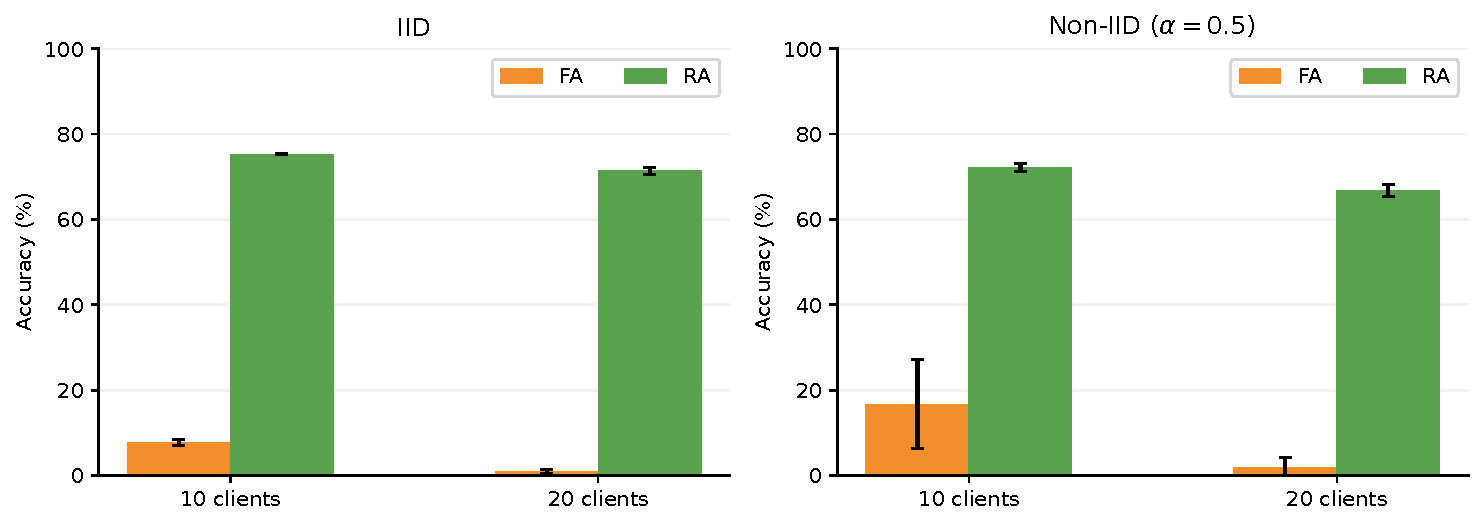
\includegraphics[width=\linewidth]{additional_clients.pdf}
\caption{Fed-EMNU with ten and twenty clients: mean $\pm$ sample SD across the same three seeds (42--44). The ten-client values use the three-seed core comparator, rather than the five-seed main mean. Partitioning and local batching change with client count; these results do not isolate a client-count-only effect.}
\label{fig:additional-clients}\end{figure}

\subsection{Retained-Only Federated Training after Revocation}

\label{sec:continuation}

To test subsequent behavioral recovery, each class-0 output of Fed-EMNU, UNSIR-style and Finetune receives five additional federated rounds using only retained data. The independently trained retained-data reference continues from its own saved state with the same additional budget. This continued reference is not a newly initialized retraining run. CIFAR-10/ResNet18, ten clients, IID and Dirichlet $\alpha=0.5$, seeds 42--44 are used.

Class 0 remains quarantined at every client throughout continuation. Each new round selects four clients with a common seed-specific schedule generated from seed $+70000$, and applies five local epochs with fresh Adam at 0.01 and batch size 128. Local shuffling uses seed $+50000+10t+i$ for zero-based round $t$ and client $i$. Each continuation loads the corresponding parent state. Parent and final accuracy are recomputed from predictions; attacks share historical-member splits and use the same declared calibration procedure. TV is against the continued reference. Values are mean $\pm$ sample SD, $n=3$.

\begin{table}[H]\centering\footnotesize\setlength{\tabcolsep}{4pt}
\caption{IID retained-only continuation. Final accuracy and final-minus-parent changes in percentage points; mean $\pm$ sample SD.}
\label{tab:continuation-iid}
\begin{tabular}{lrrrr}\toprule Parent & FA (\%) & RA (\%) & $\Delta$FA (pp) & $\Delta$RA (pp)\\\midrule
Retained reference & $0.00 \pm 0.00$ & $74.92 \pm 0.44$ & $0.00 \pm 0.00$ & $0.58 \pm 0.33$\\
Finetune & $0.00 \pm 0.00$ & $75.25 \pm 0.21$ & $-77.90 \pm 0.26$ & $1.29 \pm 0.38$\\
Fed-EMNU & $0.00 \pm 0.00$ & $74.83 \pm 0.13$ & $-7.70 \pm 0.70$ & $-0.46 \pm 0.17$\\
UNSIR-style & $0.03 \pm 0.06$ & $75.27 \pm 0.16$ & $-4.33 \pm 1.56$ & $0.48 \pm 0.28$\\
\bottomrule\end{tabular}\end{table}
\begin{table}[H]\centering\footnotesize\setlength{\tabcolsep}{4pt}
\caption{IID retained-only continuation. Final membership AUC and total-variation distance from the continued reference; mean $\pm$ sample SD.}
\label{tab:continuation-iid-compute}
\begin{tabular}{lrr}\toprule Parent & Target AUC & TV\\\midrule
Retained reference & $0.500 \pm 0.017$ & 0 (self)\\
Finetune & $0.647 \pm 0.007$ & $0.252 \pm 0.006$\\
Fed-EMNU & $0.628 \pm 0.024$ & $0.253 \pm 0.003$\\
UNSIR-style & $0.633 \pm 0.006$ & $0.250 \pm 0.005$\\
\bottomrule\end{tabular}\end{table}

Under IID, Fed-EMNU target AUC changes from $0.614 \pm 0.021$ to $0.628 \pm 0.024$, while the continued reference has AUC $0.500 \pm 0.017$. The final paired AUC difference from the continued reference is $0.128 \pm 0.039$. Continued training is additional compute: Fed-EMNU continuation takes $46.64 \pm 1.96$ s, excluding the original unlearning event, evaluation and real transport. The continuation wrapper does not measure transport payload; its empty communication record must not be interpreted as zero network traffic.

\begin{table}[H]\centering\footnotesize\setlength{\tabcolsep}{4pt}
\caption{Non-IID retained-only continuation. Final accuracy and final-minus-parent changes in percentage points; mean $\pm$ sample SD.}
\label{tab:continuation-noniid}
\begin{tabular}{lrrrr}\toprule Parent & FA (\%) & RA (\%) & $\Delta$FA (pp) & $\Delta$RA (pp)\\\midrule
Retained reference & $0.00 \pm 0.00$ & $68.44 \pm 1.76$ & $0.00 \pm 0.00$ & $-0.97 \pm 1.96$\\
Finetune & $0.10 \pm 0.10$ & $69.94 \pm 0.19$ & $-68.17 \pm 7.16$ & $-1.06 \pm 0.48$\\
Fed-EMNU & $0.37 \pm 0.64$ & $69.99 \pm 0.98$ & $-16.37 \pm 9.79$ & $-2.16 \pm 1.68$\\
UNSIR-style & $0.10 \pm 0.17$ & $70.35 \pm 0.28$ & $-4.73 \pm 4.15$ & $-0.28 \pm 1.01$\\
\bottomrule\end{tabular}\end{table}
\begin{table}[H]\centering\footnotesize\setlength{\tabcolsep}{4pt}
\caption{Non-IID retained-only continuation. Final membership AUC and total-variation distance from the continued reference; mean $\pm$ sample SD.}
\label{tab:continuation-noniid-compute}
\begin{tabular}{lrr}\toprule Parent & Target AUC & TV\\\midrule
Retained reference & $0.513 \pm 0.037$ & 0 (self)\\
Finetune & $0.603 \pm 0.017$ & $0.300 \pm 0.022$\\
Fed-EMNU & $0.616 \pm 0.030$ & $0.300 \pm 0.023$\\
UNSIR-style & $0.605 \pm 0.013$ & $0.299 \pm 0.019$\\
\bottomrule\end{tabular}\end{table}

Under Non-IID, Fed-EMNU target AUC changes from $0.598 \pm 0.005$ to $0.616 \pm 0.030$, while the continued reference has AUC $0.513 \pm 0.037$. The final paired AUC difference from the continued reference is $0.104 \pm 0.015$. Continued training is additional compute: Fed-EMNU continuation takes $42.63 \pm 3.81$ s, excluding the original unlearning event, evaluation and real transport. The continuation wrapper does not measure transport payload; its empty communication record must not be interpreted as zero network traffic.

Class-0 FA increases in 0 of the six Fed-EMNU continuations. This is a finite-horizon behavioral check under strict quarantine, not evidence of equality to retraining or a privacy guarantee. In particular, suppressed target accuracy can coexist with membership scores different from the continued reference. This experiment does not test reintroduction of revoked data, arbitrary future training, device failures or long request streams. No general no-relearning claim follows.

\begin{figure}[htbp]\centering
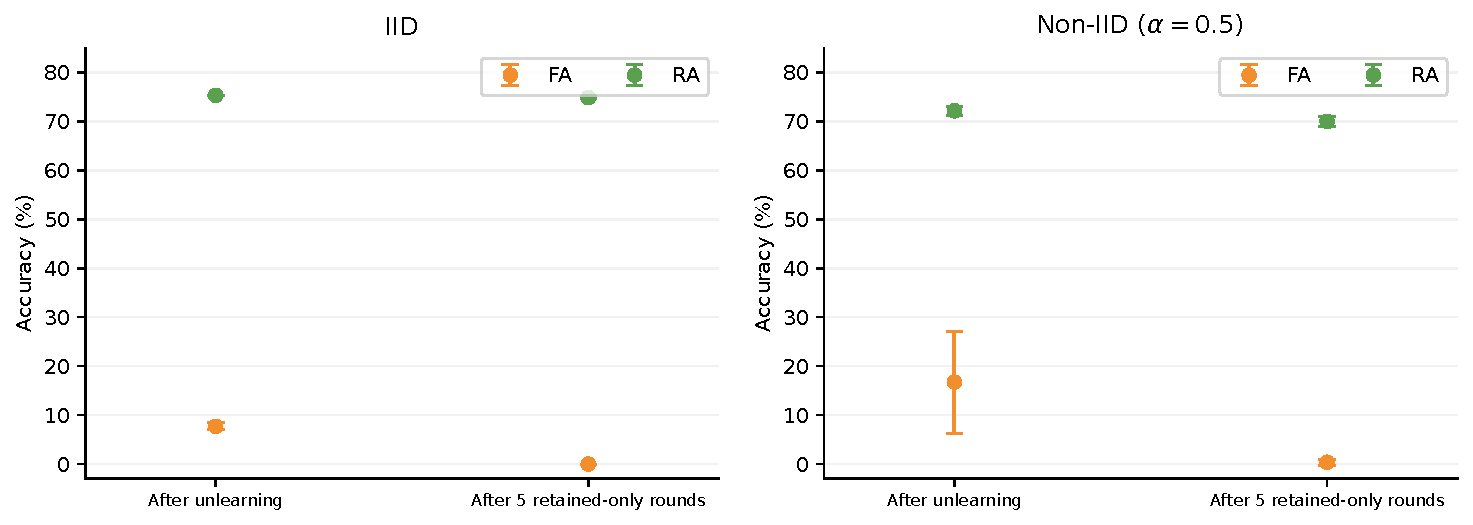
\includegraphics[width=\linewidth]{additional_continuation.pdf}
\caption{Fed-EMNU FA and RA immediately after unlearning and after five retained-only FL rounds, mean $\pm$ sample SD across three seeds. Only these two endpoints are shown; no intermediate-round trajectory is inferred. Class 0 remains quarantined; the comparison does not establish unrestricted future-training behavior.}
\label{fig:additional-continuation}\end{figure}


\section{Controlled Comparisons and Timing Details}
\label{sec:controlled-details}
The following three-seed controls and technical timing repeats supplement
the concise interpretation in Section~\ref{sec:controlled-summary}.
\subsection{Controlled Noise Objectives and Event Aggregation}
\label{sec:round2-controls}
The second-round controls use the original CIFAR-10/ResNet18 checkpoints and
references for seeds 42--44 in both partitions. All controls retain the full
local retained set and use the same random ordering, local learning rates and
attack splits. This explicitly removes the mode-dependent automatic ordering
used in the primary recipes. The high budget has 80 server noise steps and
three repair epochs; the low budget has 40 steps and one repair epoch. One
impair epoch is used throughout. At each budget, Fed and UNSIR differ only in
the norm penalty defined in Section~\ref{sec:noise}. Realized local optimizer
steps are identical within each paired budget. These are matched update
budgets, not enforced equal wall-clock times or the centralized UNSIR protocol.
The Gaussian control omits noise optimization; equal weights changes only
request-event aggregation. Both otherwise follow Fed high. Gaussian saves
server steps and is not equal compute. No result was used to tune a budget.
Values are mean $\pm$ sample SD across three paired scientific seeds.
\begin{table}[H]\centering\footnotesize\setlength{\tabcolsep}{4pt}
\caption{Second-round IID controls ($n=3$). Predictive behavior; FA/RA are percent, AUC/TV are probability units. Entries are mean $\pm$ sample SD.}
\label{tab:round2-iid}
\begin{tabular}{lrrrr}\toprule Variant & FA (\%) & RA (\%) & Target AUC & TV\\\midrule
Fed high & $7.70 \pm 0.70$ & $75.29 \pm 0.05$ & $0.614 \pm 0.021$ & $0.255 \pm 0.003$\\
UNSIR high & $7.50 \pm 1.21$ & $75.23 \pm 0.37$ & $0.615 \pm 0.014$ & $0.254 \pm 0.004$\\
Fed low & $5.07 \pm 0.45$ & $74.79 \pm 0.49$ & $0.594 \pm 0.022$ & $0.260 \pm 0.007$\\
UNSIR low & $4.37 \pm 1.56$ & $74.79 \pm 0.19$ & $0.598 \pm 0.027$ & $0.262 \pm 0.005$\\
Gaussian & $11.17 \pm 2.75$ & $75.72 \pm 0.06$ & $0.643 \pm 0.010$ & $0.252 \pm 0.003$\\
Equal weights & $7.70 \pm 0.70$ & $75.29 \pm 0.05$ & $0.614 \pm 0.021$ & $0.255 \pm 0.003$\\
\bottomrule\end{tabular}\end{table}
\begin{table}[H]\centering\footnotesize\setlength{\tabcolsep}{4pt}
\caption{Second-round IID controls ($n=3$). Realized local update counts and actual execution time in seconds; server noise-step counts are specified in the text. Entries are mean $\pm$ sample SD.}
\label{tab:round2-iid-compute}
\begin{tabular}{lrr}\toprule Variant & Local steps & Exec. (s)\\\midrule
Fed high & $1640 \pm 0$ & $21.47 \pm 0.52$\\
UNSIR high & $1640 \pm 0$ & $21.38 \pm 0.69$\\
Fed low & $920 \pm 0$ & $12.58 \pm 0.18$\\
UNSIR low & $920 \pm 0$ & $11.97 \pm 0.36$\\
Gaussian & $1640 \pm 0$ & $21.22 \pm 0.30$\\
Equal weights & $1640 \pm 0$ & $22.44 \pm 0.47$\\
\bottomrule\end{tabular}\end{table}
\begin{table}[H]\centering\footnotesize\setlength{\tabcolsep}{4pt}
\caption{Second-round Non-IID controls ($n=3$). Predictive behavior; FA/RA are percent, AUC/TV are probability units. Entries are mean $\pm$ sample SD.}
\label{tab:round2-noniid}
\begin{tabular}{lrrrr}\toprule Variant & FA (\%) & RA (\%) & Target AUC & TV\\\midrule
Fed high & $13.97 \pm 13.19$ & $72.09 \pm 1.00$ & $0.604 \pm 0.013$ & $0.319 \pm 0.007$\\
UNSIR high & $14.20 \pm 13.63$ & $72.56 \pm 1.12$ & $0.591 \pm 0.006$ & $0.317 \pm 0.008$\\
Fed low & $4.50 \pm 2.84$ & $70.27 \pm 1.30$ & $0.585 \pm 0.011$ & $0.333 \pm 0.016$\\
UNSIR low & $4.83 \pm 4.32$ & $70.63 \pm 1.07$ & $0.583 \pm 0.002$ & $0.329 \pm 0.013$\\
Gaussian & $11.47 \pm 0.90$ & $72.42 \pm 0.82$ & $0.626 \pm 0.006$ & $0.316 \pm 0.017$\\
Equal weights & $13.37 \pm 13.18$ & $71.20 \pm 0.80$ & $0.596 \pm 0.019$ & $0.336 \pm 0.014$\\
\bottomrule\end{tabular}\end{table}
\begin{table}[H]\centering\footnotesize\setlength{\tabcolsep}{4pt}
\caption{Second-round Non-IID controls ($n=3$). Realized local update counts and actual execution time in seconds; server noise-step counts are specified in the text. Entries are mean $\pm$ sample SD.}
\label{tab:round2-noniid-compute}
\begin{tabular}{lrr}\toprule Variant & Local steps & Exec. (s)\\\midrule
Fed high & $1628 \pm 0$ & $23.30 \pm 0.46$\\
UNSIR high & $1628 \pm 0$ & $22.26 \pm 0.57$\\
Fed low & $914 \pm 0$ & $13.13 \pm 0.07$\\
UNSIR low & $914 \pm 0$ & $12.51 \pm 0.47$\\
Gaussian & $1628 \pm 0$ & $21.85 \pm 0.28$\\
Equal weights & $1628 \pm 0$ & $21.92 \pm 1.23$\\
\bottomrule\end{tabular}\end{table}
\textbf{Objective and budget controls.} At the high budget, the paired
Fed-minus-UNSIR RA difference is $0.063\pm0.371$ percentage points under IID
and $-0.463\pm0.361$ under Non-IID. At the low budget, the corresponding
differences are $-0.004\pm0.306$ and $-0.356\pm0.222$ points. Paired FA
differences are $0.200\pm1.735$ and $-0.233\pm0.451$ points at the high
budget, and $0.700\pm1.480$ and $-0.333\pm1.856$ at the low budget.
Thus, the matched-update-budget controls do not support a consistent retained-utility
advantage of the unsquared whole-tensor penalty. In the three Non-IID pairs,
the squared-penalty adaptation has higher retained accuracy at both budgets.
The primary recipe's RA advantage therefore cannot be attributed to the
Fed-EMNU penalty alone. These descriptive results do not establish population
equivalence or isolate the separate effects of increasing noise and repair
budgets, which change together between low and high.

\textbf{Optimized versus Gaussian inputs.} Fed high minus Gaussian changes
FA by $-3.467\pm3.200$ points under IID, but by $2.500\pm12.322$ under
Non-IID. RA differences are $-0.430\pm0.107$ and $-0.330\pm0.195$ points.
Optimization improves mean class suppression in this IID control but does
not establish a robust benefit across partitions. The large Non-IID variation
and the absence of a retained-utility gain argue against claiming that noise
optimization is uniformly effective for these accuracy metrics. Target attack
AUC decreases relative to Gaussian inputs by $0.029\pm0.012$ under IID and
$0.022\pm0.018$ under Non-IID, with a decrease in all three pairs in each
partition. This is a favorable outcome for the declared attack, alongside the
mixed accuracy results; it does not establish a privacy guarantee. Neither noise choice demonstrates
verified deletion; the reported target attack and reference distances remain
necessary diagnostics.

\textbf{Event aggregation.} Equal retained counts make weighted and equal
event aggregation identical under IID; saved posterior arrays are exactly
equal in all three pairs. Under Non-IID, retained-count weighting increases
RA by $0.896\pm0.224$ points and FA by $0.600\pm0.557$ relative to equal
weighting. This supports a limited utility--suppression trade-off for the
stated event rule, not a general aggregation advantage. It does not resolve
the omission of separate repair contributions from non-target holders in
sparse-owner settings.

Taken together, the new controls strengthen attribution and expose negative
evidence. They support describing a particular empirical recipe and its
operating limits rather than a newly established superior noise principle.
Only three paired scientific seeds are used per partition; no multiple-testing
adjustment or formal equivalence claim is made.

\subsection{Robust Timing Summaries and Outlier Investigation}
\label{sec:round2-timing}
Table~\ref{tab:robust-time} supplements the original mean/SD tables with medians
and quartiles from the same five primary seeds, retaining every observation.
Quartiles use linear interpolation. These seed-level times include changes in
partition/schedule and execution conditions; they are not identical-workload
technical repetitions. Historical hardware telemetry is unavailable, so a
specific cause of the old outlier cannot be established from saved times.
\begin{table}[H]\centering\small
\caption{Original primary compute/serialization time in seconds, five seeds;
median [first, third quartile]. Evaluation and network transport excluded.}
\label{tab:robust-time}\begin{tabular}{llrr}\toprule
Setting & Method & Median [Q1, Q3] & Range\\\midrule
IID & Retrain & 431.25 [428.54, 477.27] & 425.97--651.38\\
IID & Fed-EMNU & 20.20 [20.00, 21.98] & 19.54--30.44\\
IID & UNSIR-style & 11.81 [11.76, 14.44] & 11.32--17.36\\
Non-IID & Retrain & 427.62 [424.71, 429.82] & 420.10--2310.15\\
Non-IID & Fed-EMNU & 22.44 [21.48, 22.52] & 21.39--114.20\\
Non-IID & UNSIR-style & 12.20 [12.03, 12.41] & 11.60--63.40\\
\bottomrule\end{tabular}\end{table}
The historical delay was not confined to Fed-EMNU: Non-IID seed 45 also
took 2310.15 s for retraining (other seeds 420.10--429.82 s)
and 63.40 s for the UNSIR-style event. This cross-method pattern
documents a broader timing anomaly, without identifying its cause.
For the Non-IID seed-42 checkpoint, three exact-recipe technical repeats
took a median 23.03 s (range 22.99--24.20 s),
compared with 22.44 s in the original session.
The maximum posterior difference from that original result was 0;
the maximum predicted-label disagreement was 0.000\%.
For the Non-IID seed-45 checkpoint, three exact-recipe technical repeats
took a median 25.76 s (range 25.48--26.13 s),
compared with 114.20 s in the original session.
The maximum posterior difference from that original result was 0;
the maximum predicted-label disagreement was 0.000\%.
These repeats use the current driver/session and are reported separately,
without replacing or pooling the historical measurements. They test whether
the saved workload consistently reproduces the large delay, but cannot identify
the historical cause. Three repeats per checkpoint are technical replicates,
not additional independent seeds. Compute time still excludes end-to-end
federated transport, energy and deployment overhead.

\subsection{Common Wall-Clock Caps}
\label{sec:walltime}
To supplement matched update counts, we compare time-capped adaptations of the
two original recipes at 10, 20, 30 and 40 seconds on the same GPU, checkpoints,
retained-data ordering and references (three seeds, both partitions). The
noise and maximum repair budgets remain 80 steps/three epochs for Fed-EMNU and
40 steps/one epoch for UNSIR-style. Method order is counterbalanced by seed
and budget. No test outcome chooses a configuration or stopping point.

After noise generation, a predefined reserve of the larger of 0.5 seconds and
15\% of the total cap is withheld for non-training overhead. The remaining
local-training time is divided equally across all affected clients. Each
client divides its allocation between impair and repair in ratio
$1:\text{repair epochs}$. Updates stop at synchronized minibatch boundaries;
the largest previous minibatch duration is reserved before another batch.
Original epoch limits also apply: recipes finishing early receive no padding
or extra training. Total observed time includes noise, local updates, model
copies, selection, aggregation and final serialization, excluding evaluation
and network transport. Per-batch synchronization introduces monitoring overhead.
These controls compare common maximum resources under a specified scheduler;
they do not establish an optimal allocation or identical consumed time.
\begin{table}[htbp]\centering\footnotesize\setlength{\tabcolsep}{4pt}
\caption{Common maximum wall-clock caps, IID, three seeds. $T_{\max}$ is the imposed upper bound; Exec. is actual execution time in seconds, not padded to the cap.}\label{tab:walltime-iid}
\begin{tabular}{rlrrrrr}\toprule $T_{\max}$ (s) & Recipe & FA (\%) & RA (\%) & Target AUC & TV & Exec. (s)\\\midrule
10 & Fed-EMNU & $15.10 \pm 2.80$ & $75.02 \pm 0.15$ & $0.626 \pm 0.025$ & $0.268 \pm 0.002$ & $8.91 \pm 0.10$\\
10 & UNSIR-style & $8.67 \pm 5.14$ & $73.61 \pm 0.26$ & $0.602 \pm 0.026$ & $0.282 \pm 0.006$ & $8.90 \pm 0.08$\\
20 & Fed-EMNU & $7.90 \pm 0.85$ & $75.22 \pm 0.08$ & $0.620 \pm 0.022$ & $0.262 \pm 0.001$ & $17.35 \pm 0.06$\\
20 & UNSIR-style & $4.23 \pm 1.26$ & $74.74 \pm 0.07$ & $0.600 \pm 0.025$ & $0.262 \pm 0.004$ & $14.52 \pm 0.24$\\
30 & Fed-EMNU & $7.97 \pm 1.66$ & $75.27 \pm 0.19$ & $0.618 \pm 0.019$ & $0.256 \pm 0.004$ & $23.36 \pm 0.70$\\
30 & UNSIR-style & $4.37 \pm 1.56$ & $74.79 \pm 0.19$ & $0.598 \pm 0.027$ & $0.262 \pm 0.005$ & $14.64 \pm 0.62$\\
40 & Fed-EMNU & $7.43 \pm 1.50$ & $75.18 \pm 0.21$ & $0.610 \pm 0.022$ & $0.256 \pm 0.002$ & $25.56 \pm 1.16$\\
40 & UNSIR-style & $4.37 \pm 1.56$ & $74.79 \pm 0.19$ & $0.598 \pm 0.027$ & $0.262 \pm 0.005$ & $14.50 \pm 0.25$\\
\bottomrule\end{tabular}\end{table}
\begin{table}[htbp]\centering\footnotesize\setlength{\tabcolsep}{4pt}
\caption{Common maximum wall-clock caps, Non-IID, three seeds. $T_{\max}$ is the imposed upper bound; Exec. is actual execution time in seconds, not padded to the cap.}\label{tab:walltime-noniid}
\begin{tabular}{rlrrrrr}\toprule $T_{\max}$ (s) & Recipe & FA (\%) & RA (\%) & Target AUC & TV & Exec. (s)\\\midrule
10 & Fed-EMNU & $15.27 \pm 10.10$ & $71.01 \pm 0.98$ & $0.610 \pm 0.013$ & $0.325 \pm 0.011$ & $8.78 \pm 0.04$\\
10 & UNSIR-style & $5.20 \pm 3.44$ & $66.51 \pm 1.41$ & $0.575 \pm 0.003$ & $0.373 \pm 0.007$ & $8.57 \pm 0.26$\\
20 & Fed-EMNU & $12.80 \pm 10.62$ & $71.80 \pm 1.30$ & $0.611 \pm 0.022$ & $0.322 \pm 0.016$ & $15.65 \pm 0.43$\\
20 & UNSIR-style & $4.80 \pm 4.87$ & $69.99 \pm 0.84$ & $0.577 \pm 0.001$ & $0.339 \pm 0.011$ & $13.90 \pm 0.67$\\
30 & Fed-EMNU & $13.17 \pm 10.26$ & $71.86 \pm 0.89$ & $0.609 \pm 0.020$ & $0.320 \pm 0.015$ & $21.27 \pm 0.93$\\
30 & UNSIR-style & $4.43 \pm 4.13$ & $70.57 \pm 1.14$ & $0.582 \pm 0.003$ & $0.328 \pm 0.011$ & $15.55 \pm 1.00$\\
40 & Fed-EMNU & $13.37 \pm 8.98$ & $72.19 \pm 0.75$ & $0.605 \pm 0.020$ & $0.318 \pm 0.011$ & $24.62 \pm 0.90$\\
40 & UNSIR-style & $4.83 \pm 4.32$ & $70.63 \pm 1.07$ & $0.583 \pm 0.002$ & $0.329 \pm 0.013$ & $15.48 \pm 1.00$\\
\bottomrule\end{tabular}\end{table}
All 48 events were checked against their requested caps: 0
events exceeded the cap. The stage records contain 0 zero-update stages.
FA/RA are recomputed from saved predictions; paired comparisons use the
same checkpoints, selections and attack splits. Exact update counts and client
stage times are recorded in the generated CSV and traces; the public release
provides per-event step counts and actual-time metrics, while raw traces must
be regenerated. The three seeds
per cell limit inference. Truncation changes stage completion and thus the
original recipes; these results cannot be substituted for their unrestricted
defaults or used as proof of general superiority at every time allocation.
Across the tested caps, Fed-EMNU has higher mean retained accuracy, but also
higher mean target accuracy and target attack AUC than the UNSIR-style recipe.
Fed-minus-UNSIR RA differences at 10/20/30/40 seconds are respectively
1.41/0.49/0.48/0.39 percentage points under IID and
4.50/1.81/1.29/1.56 points under Non-IID. Corresponding FA differences are
6.43/3.67/3.60/3.07 points and 10.07/8.00/8.73/8.53 points.
Target attack AUC differences range from 0.013 to 0.025 under IID and
0.022 to 0.035 under Non-IID. Thus the retained-utility gain comes with weaker
target suppression and greater distinguishability under the declared attack;
these results do not establish uniform superiority or a privacy advantage.

At wider caps, UNSIR-style often finishes its prescribed recipe early, while
Fed-EMNU continues more of its larger repair budget. This is a common-resource
cap comparison of the specified recipes, rather than proof that every recipe
uses the same actual time or that its budget allocation is optimal. The common
update-count controls remain necessary for separating the noise objective from
the recipe budget. Hardware-dependent minibatch stopping also limits exact
cross-device replication of the achieved step counts. Full per-seed outcomes,
paired SDs and actual-time metrics are public; replay commands regenerate
the excluded raw stage traces.



\clearpage
\reftitle{References}
\externalbibliography{yes}
\bibliography{references}
\end{document}

